\documentclass[a4paper, 12pt]{article}
\usepackage[a4paper,top=1.5cm, bottom=1.5cm, left=1cm, right=1cm]{geometry}
\usepackage{cmap}					% поиск в PDF
\usepackage{mathtext} 				% русские буквы в формулах
\usepackage[T2A]{fontenc}			% кодировка
\usepackage[utf8]{inputenc}			% кодировка исходного текста
\usepackage[english,russian]{babel}	% локализация и переносы

\usepackage{amsmath,amssymb}
\usepackage{indentfirst}
\usepackage{longtable}
\usepackage{graphicx}
\usepackage{array}
\usepackage{float}

\usepackage{floatflt}
\usepackage{wrapfig}
\usepackage{siunitx} % Required for alignment
\usepackage{subfigure}
\usepackage{multirow}
\usepackage{rotating}
\usepackage{caption}

\graphicspath{{.}}


\title{\begin{center}Лабораторная работа №3.6.1\end{center}
Спектральный анализ электрических сигналов}
\author{Рожков А. В.}
\date{\today}

\begin{document}
    \pagenumbering{gobble}
    \maketitle
    \newpage
    \pagenumbering{arabic}
    \renewcommand*{\thesubsection}{\thesection.\Alph{subsection}}

    \textbf{Цель работы:} изучить спектры сигналов различной формы и влияние параметров сигнала на вид соответствующих спектров; проверить справедливость соотношений неопределённостей; познакомиться с работой спектральных фильтров на примере RC-цепочки

    \textbf{В работе используются:} генератор сигналов произвольной формы, цифровой осциллограф с функцией быстрого преобразования Фурье или цифровой USB-осциллограф, подключённый к персональному компьютеру.

    \section{Теоретическое введение}

        \subsection{Разложение сложных сигналов на периодические колебания}
            Представление периодического сигнала в виде суммы гармонических сигналов называется разложением в ряд Фурье.

	        Пусть заданная функция $f(t)$ периодически повторяется с частотой $\Omega_{1}=\dfrac{2\pi}{T},$ где $T$ - период повторения. Ее разложение в ряд Фурье имеет вид
            \begin{equation}
                f(t)=\dfrac{a_{0}}{2}+ \sum\limits_{n=1}^\infty [a_{n}\cos(n \Omega_{1}t)+b_{n}\sin(n \Omega_{1} t) ]
                \label{eq1}
            \end{equation}
		    Здесь $\dfrac{a_{0}}{2}$ - среднее значение функции $f(t)$,

            \begin{equation}
                a_{n}=\dfrac{2}{T}\int\limits_{t_{1}}^{t_{1}+T}f(t)\cos(n \Omega_{1} t)dt,
                \label{eq2}
            \end{equation}
            \begin{equation}
                b_{n}=\dfrac{2}{T}\int\limits_{t_{1}}^{t_{1}+T}f(t)\sin(n \Omega_{1} t)dt.
                \label{eq3}
            \end{equation}

	        Рассмотрим периодические функции, которые исследуются в нашей работе.

            \subsubsection{Периодическая последовательность прямоугольных импульсов}

                (рис. 1) с амплитудой $V_{0}$, длительностью $\tau$, частотой повторения $\Omega_{1}=\dfrac{2\pi}{T},$ где $T$ - период повторения импульсов. Найдем коэффициенты разложения ряда Фурье:

                $$\dfrac{a_{0}}{2}=V_{0}\dfrac{\tau}{T},$$

                \begin{equation}
                    a_{n}=\dfrac{2}{T}\int\limits_{-\frac{\tau}{2}}^{\frac{\tau}{2}}V_{0}\cos(n \Omega_{1} t)dt=2V_{0}\dfrac{\tau}{T}\dfrac{\sin(n \Omega_{1} \frac{\tau}{2})}{n\Omega_{1}\frac{\tau}{2}} \sim \dfrac{\sin x}{x}.
                    \label{eq4}
                \end{equation}

                Поскольку наша функция четная, все коэффициенты синусоидальных гармоник $b_{n}=0$. Спектр $a_{n}$ последовательности прямоугольных импульсов представлен на рис. 2 (изображен случай, когда $T$ кратно $\tau$).

                \begin{figure}[ht]
                    \begin{minipage}[ht]{0.45\linewidth}
                        \center{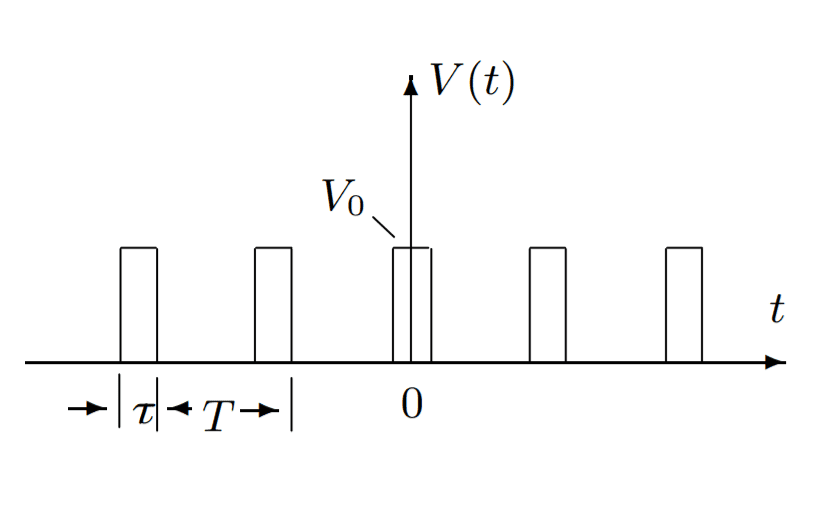
\includegraphics[width=0.9\linewidth]{img/sp1.png}}
                        \caption{Прямоугольные импульсы}
                    \end{minipage}
                    \begin{minipage}[ht]{0.45\linewidth}
                        \center{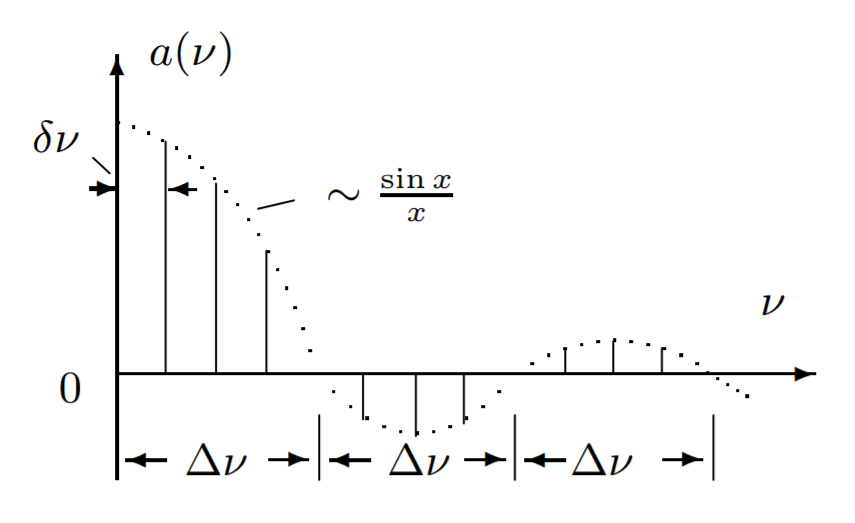
\includegraphics[width=0.9\linewidth]{img/sp2.png}}
                        \caption{Спектр последовательности прямоугольных импульсов}
                    \end{minipage}
                \end{figure}

                Назовем \textit{шириной спектра} $\Delta \omega$ расстояние от главного максимума ($\omega =0$) до первого нуля огибающей, возникающего при $n=\dfrac{2\pi}{\tau \Omega_{1}}$. При этом

                $$\Delta \omega \tau \backsimeq 2 \pi $$

                или

                \begin{equation}\label{neopr}
                    \Delta \nu \Delta t \backsimeq 1
                \end{equation}

                Полученное соотношение взаимной связи интервалов $\Delta \nu$ и $\Delta t$ является частным случаем соотношения неопределенности в квантовой механике.

            \subsubsection{Периодическая последовательность цугов}

                гармонического колебания $V_{0}\cos(\omega_{0}t)$ с длительностью цуга $\tau$ и периодом повторения $T$ (рис. 3).

                Функция $f(t)$ снова является четной относительно $t=0$. Коэффициент при $n$-й гармонике равен
                \begin{equation}
                    a_{n}=\dfrac{2}{T}\int\limits_{-\frac{\tau}{2}}^{\frac{\tau}{2}}V_{0}\cos(\omega_{0}t)\cos(n \Omega_{1} t)dt=V_{0}\dfrac{\tau}{T} \bigg(\dfrac{\sin[(\omega_{0}-n\Omega_{1})\frac{\tau}{2}]}{(\omega_{0}-n\Omega_{1})\frac{\tau}{2}}+\dfrac{\sin[(\omega_{0}+n\Omega_{1})\frac{\tau}{2}]}{(\omega_{0}+n\Omega_{1})\frac{\tau}{2}} \bigg)
                    \label{eq6}
                \end{equation}

                Зависимость для случая, когда $\frac{T}{\tau}$ равно целому числу, представлена на рис. 4. Сравнивая спектр последовательности прямоугольных импульсов и цугов мы видим, что они аналогичны, но их максимумы сдвинуты по частоте на величину $\omega_{0}$.

                \begin{figure}[ht]
                    \begin{minipage}[ht]{0.45\linewidth}
                        \center{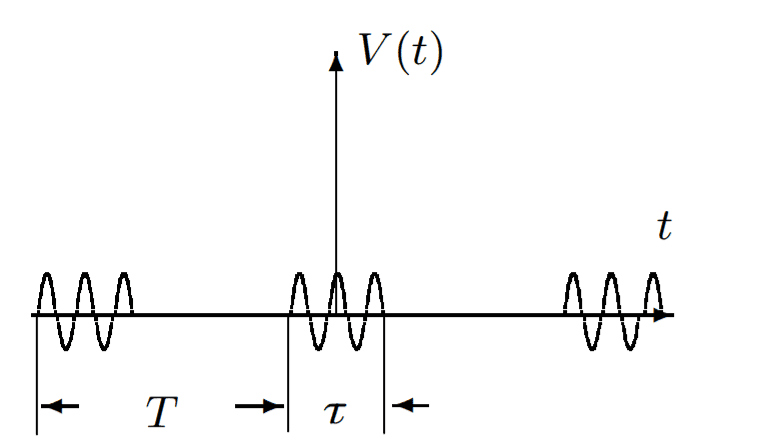
\includegraphics[width=0.9\linewidth]{img/sp3.png}}
                        \caption{Последовательность цугов}
                    \end{minipage}
                    \begin{minipage}[ht]{0.45\linewidth}
                        \center{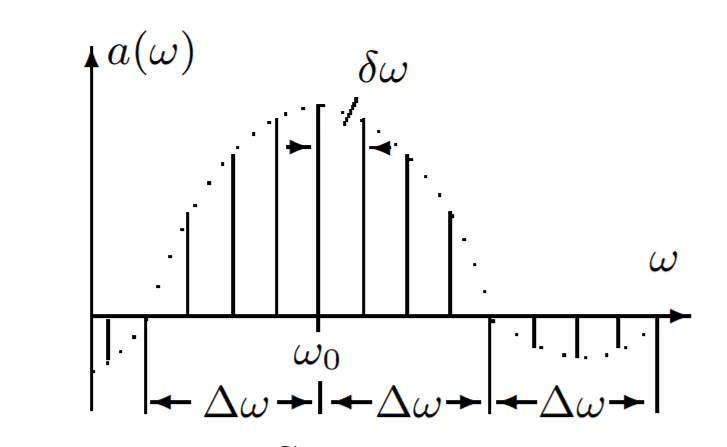
\includegraphics[width=0.9\linewidth]{img/sp4.png}}
                        \caption{Спектр последовательности цугов}
                    \end{minipage}
                \end{figure}

            \subsubsection{Амплитудно-модулированные колебания}

                Рассмотрим гармонические колебания высокой частоты $\omega_{0}$ , амплитуда которых медленно меняется по гармоническому закону с частотой $\Omega$ ($\Omega \ll \omega_{0})$) (рис. 5):
                \begin{equation}
                    f(t)=A_{0}[1+m\cos\Omega t]\cos \omega_{0}t
                    \label{eq7}
                \end{equation}

                Коэффициент $m$ называют \textbf{глубиной модуляции}. При $m<1$ амплитуда колебаний меняется от минимальной $A_{min}=A_{0}(1-m)$ до максимальной $A_{max}=A_{0}(1+m).$ Глубина модуляции может быть представлена в виде

                \begin{equation}\label{m}
                    m=\dfrac{A_{max}-A_{min}}{A_{max}+A_{min}}
                \end{equation}

                Простым тригонометрическим преобразованием можно найти спектр амплитудно - модулированных колебаний:

                \begin{equation}\label{a}
                    f(t)=A_{0}\cos(\omega_{0} t)+\dfrac{A_{0}m}{2}\cos(\omega_{0}+\Omega)t+\dfrac{A_{0}m}{2}\cos(\omega_{0}-\Omega)t.
                \end{equation}

                \begin{figure}[ht]
                    \begin{minipage}[ht]{0.45\linewidth}
                        \center{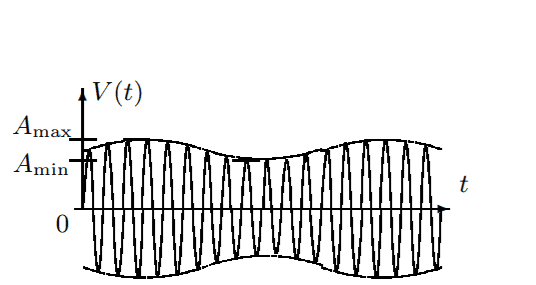
\includegraphics[width=0.9\linewidth]{img/sp5.png}}
                        \caption{Модулированные гармонические колебания}
                    \end{minipage}
                    \begin{minipage}[ht]{0.45\linewidth}
                        \center{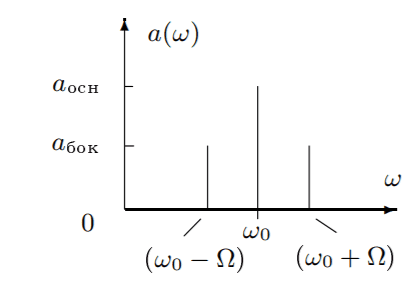
\includegraphics[width=0.9\linewidth]{img/sp6.png}}
                        \caption{Спектр модулированных гармонических колебаний}
                    \end{minipage}
                \end{figure}

                Спектр таких колебаний содержит три составляющих  основную компоненту и две боковых (рис. 6). Первое слагаемое в правой части представляет собой исходное немодулированное колебание с основной (несущей) частотой $\omega_{0}$ и амплитудой $a_{осн} = A_{0}$ . Второе и третье слагаемые соответствуют новым гармоническим колебаниям с частотами $\omega_{0} + \Omega$ и $\omega_{0} - \Omega$. Амплитуды этих двух колебаний одинаковы и составляют $\dfrac{m}{2}$ от амплитуды немодулированного колебания:

                $a_{бок} = \dfrac{A_{0}m}{2}$. Начальные фазы всех трех колебаний одинаковы.

    \section{Ход работы}

        \subsection{Исследование спектра периодической последовательности\\прямоугольных импульсов и проверка соотношений\\неопределённостей}

            \setcounter{subsubsection}{2}
            \subsubsection{Настроим прямоугольный сигнал}

                $\nu_{повт} = 1~кГц$, $\tau = T/20 = 50~мкс$

            \subsubsection{Устойчивая картина на экране осциллографа}

                Снимок экрана на рисунке \ref{plot:A.4}

                \begin{figure}[ht]
                    \begin{minipage}[ht]{0.49\linewidth}
                        \center{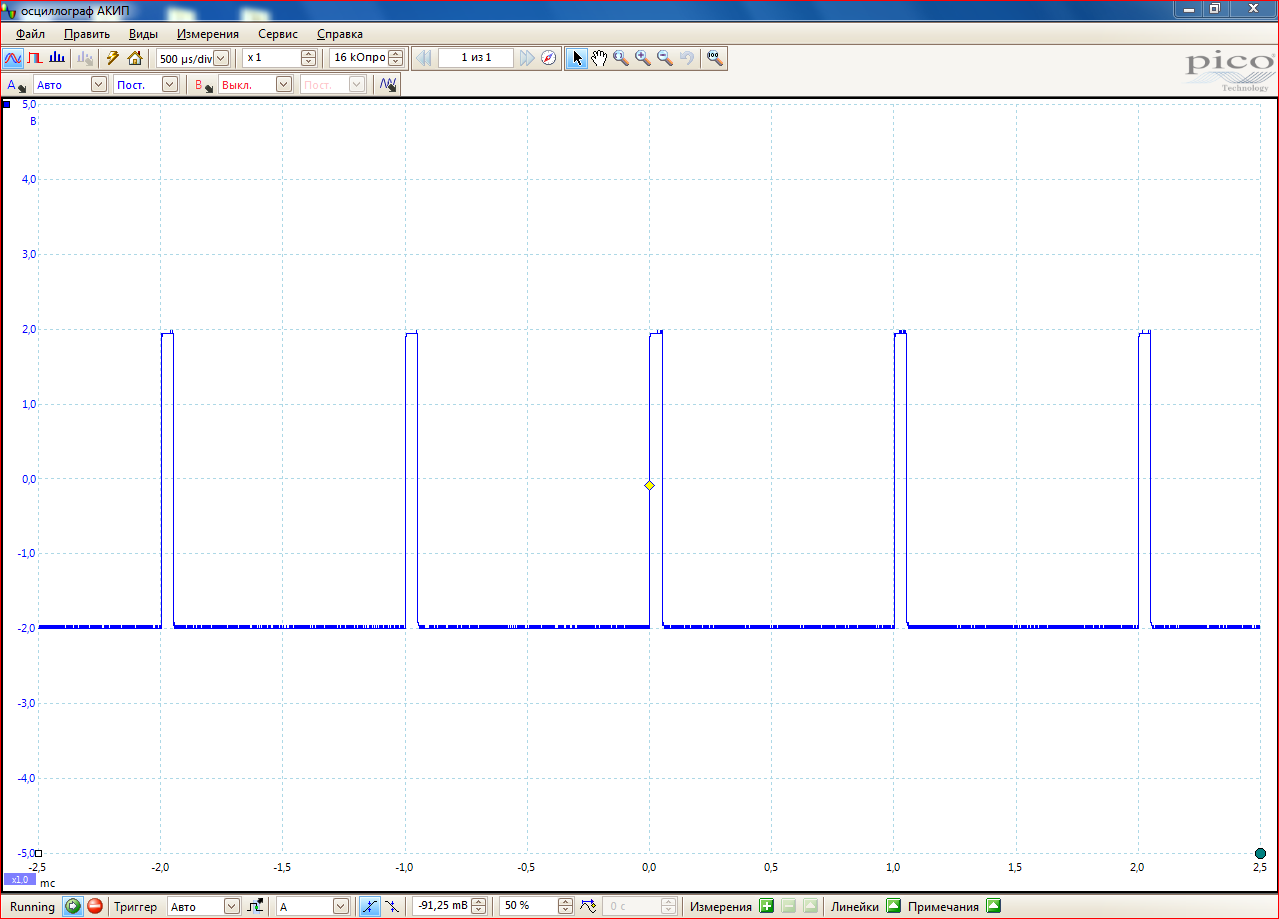
\includegraphics[width=0.95\linewidth]{img/data/A.4.png}}
                        \caption{Устойчивая картина прямоугольных импульсов}
                        \label{plot:A.4}
                    \end{minipage}
                    \begin{minipage}[ht]{0.49\linewidth}
                        \center{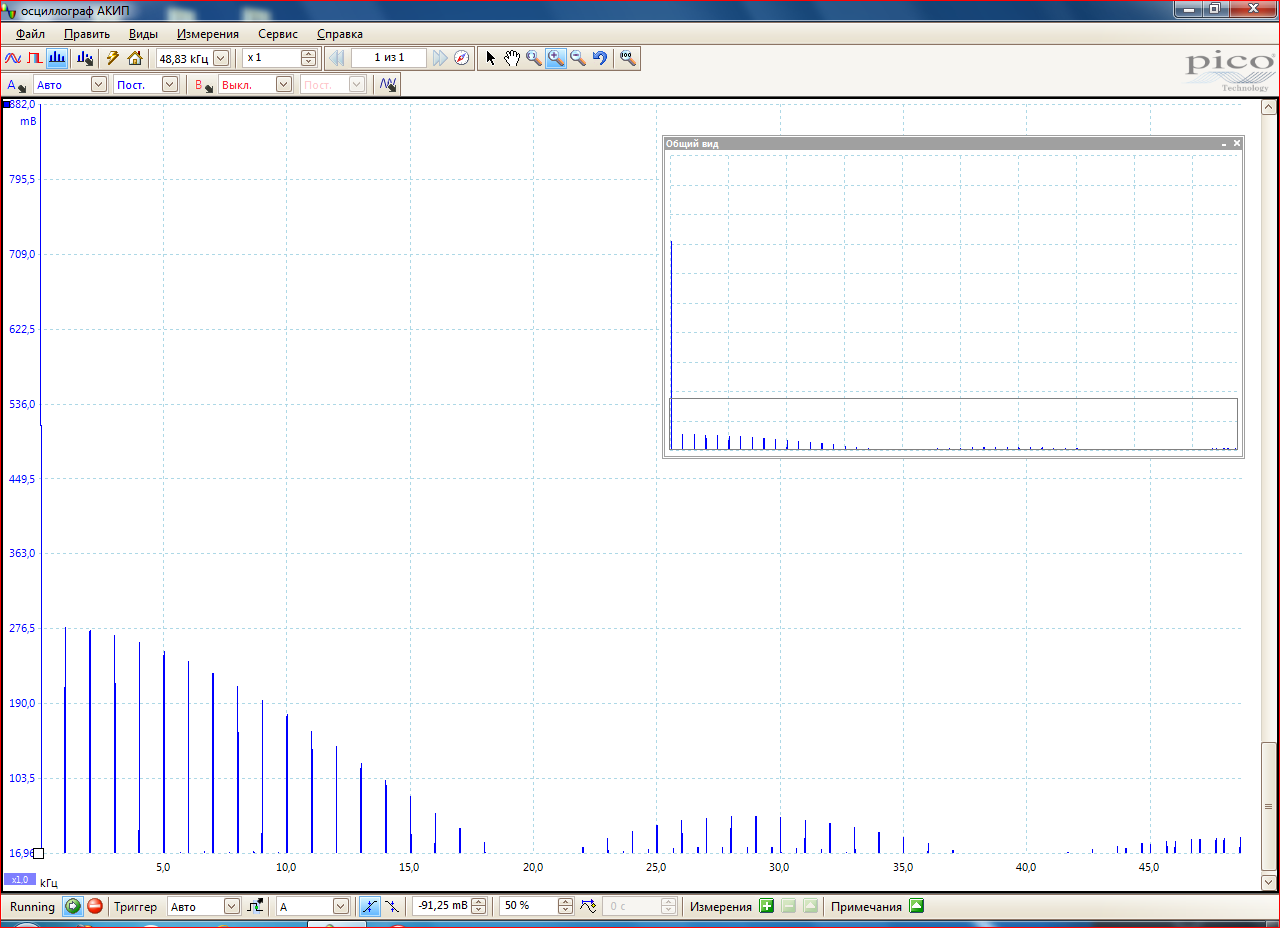
\includegraphics[width=0.95\linewidth]{img/data/A.5.png}}
                        \caption{Спектр прямоугольных импульсов (преобразование Фурье)}
                        \label{plot:A.5}
                    \end{minipage}
                \end{figure}

            \subsubsection{Спектр прямоугольного сигнала (преобразование Фурье)}

                Снимок экрана на рисунке \ref{plot:A.5}

            \subsubsection{Наблюдение изменений спектра при изменеии параметров сигнала}

                Результаты и параметра на рисунках \ref{plot:A.6.1}, \ref{plot:A.6.2}, \ref{plot:A.6.3}, \ref{plot:A.6.4}, \ref{plot:A.6.5}, \ref{plot:A.6.6}, \ref{plot:A.6.7}

                \begin{figure}[ht]
                    \begin{minipage}[ht]{0.49\linewidth}
                        \center{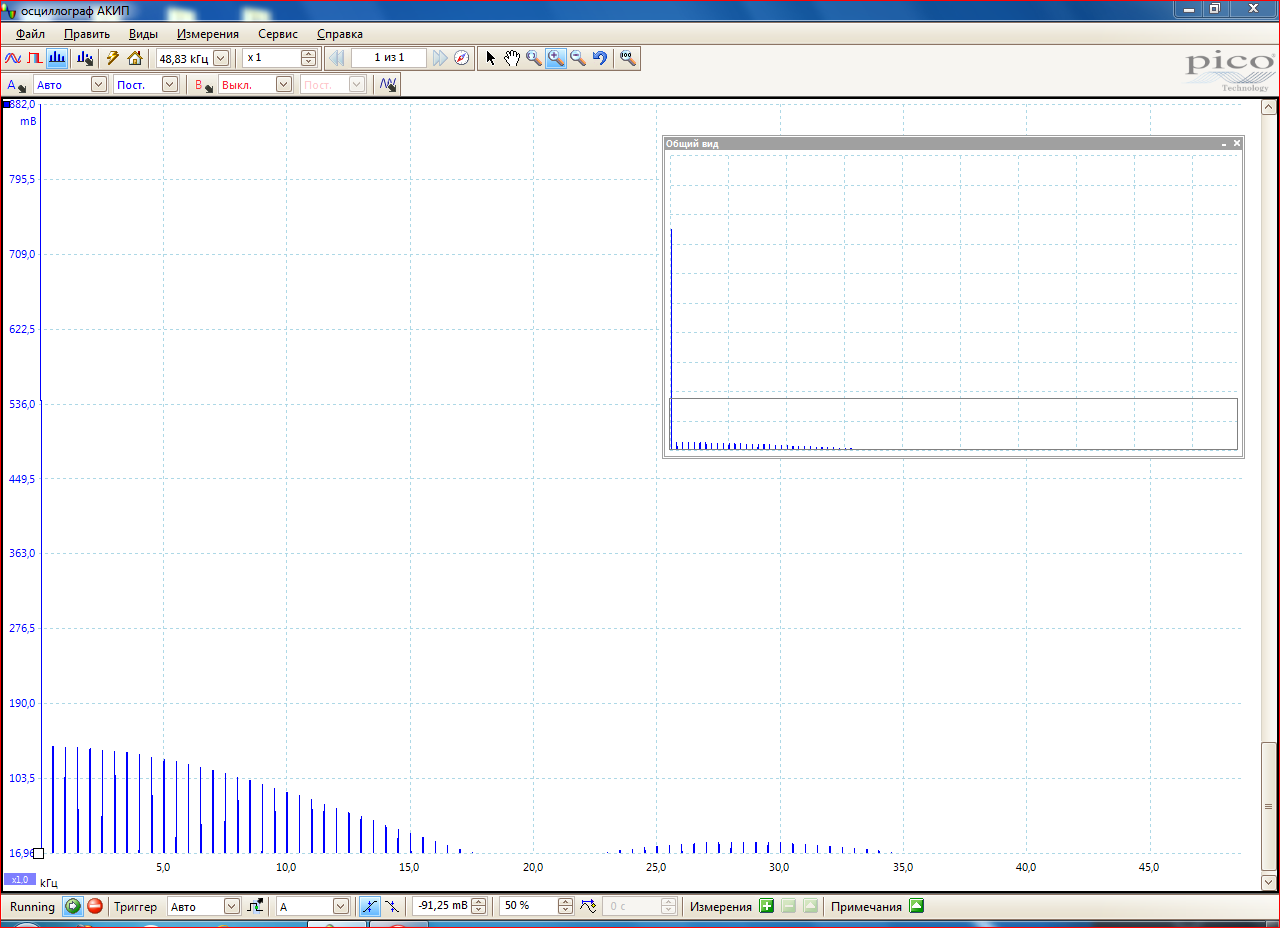
\includegraphics[width=0.95\linewidth]{img/data/A.6/0.5kHz_50us.png}}
                        \caption{Спектр прямоугольного сигнала\\($\nu_{повт} = 0.5~кГц$; $\tau = 50~мкс$)}
                        \label{plot:A.6.1}
                    \end{minipage}
                    \begin{minipage}[ht]{0.49\linewidth}
                        \center{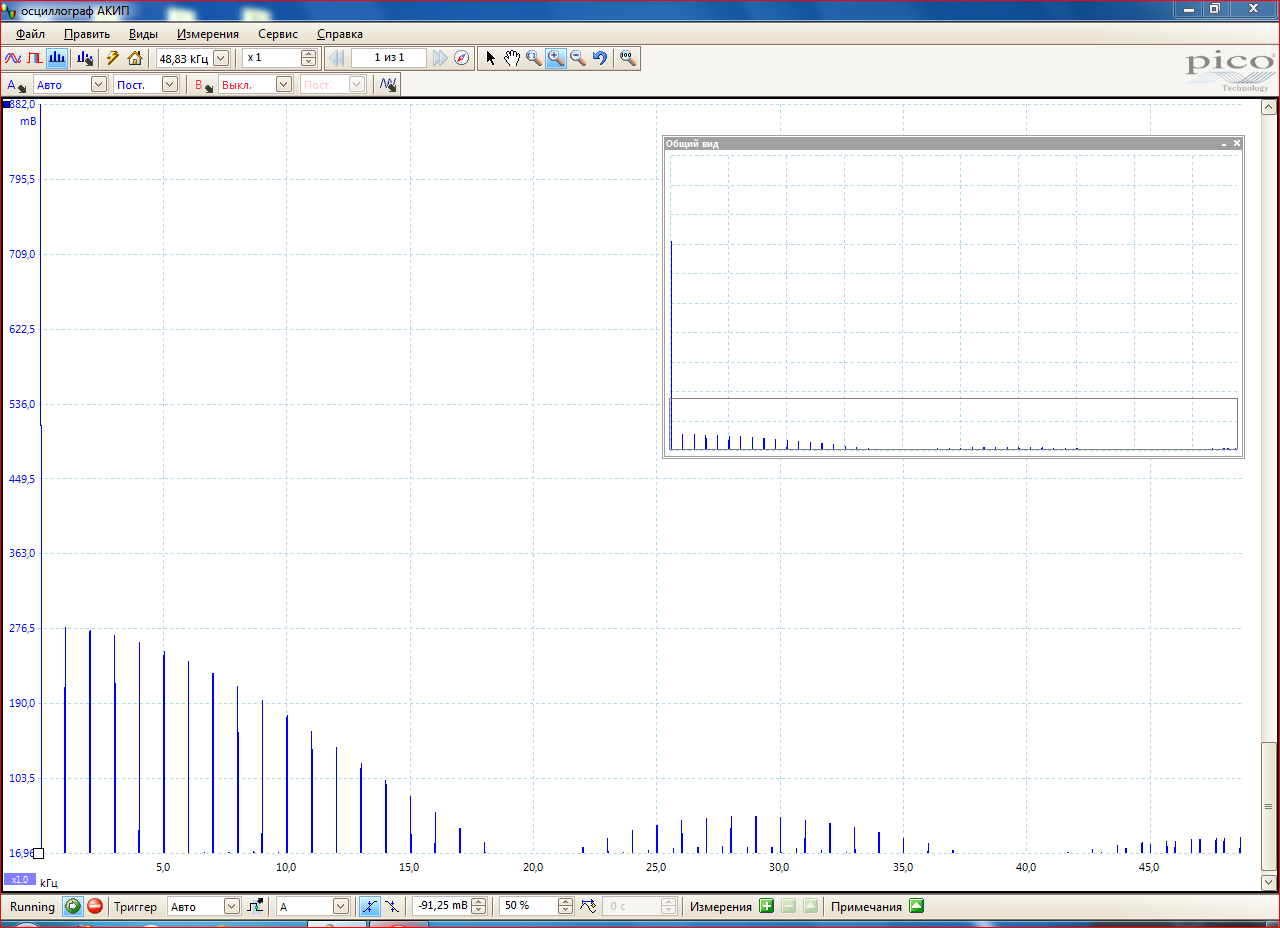
\includegraphics[width=0.95\linewidth]{img/data/A.6/1.0kHz_50us.png}}
                        \caption{Спектр прямоугольного сигнала\\($\nu_{повт} = 1~кГц$; $\tau = 50~мкс$)}
                        \label{plot:A.6.2}
                    \end{minipage}
                \end{figure}

                \begin{figure}[ht]
                    \begin{minipage}[ht]{0.49\linewidth}
                        \center{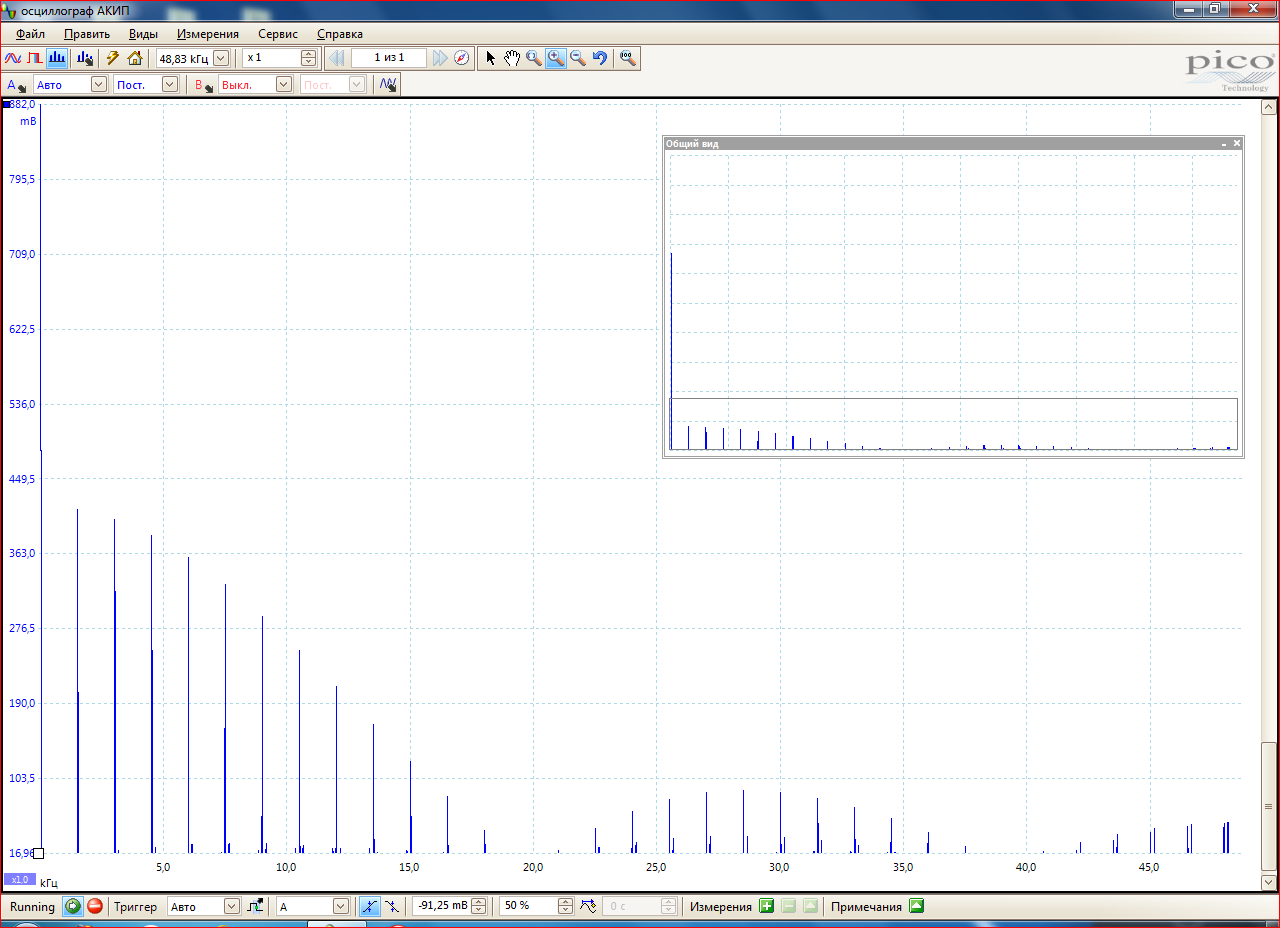
\includegraphics[width=0.95\linewidth]{img/data/A.6/1.5kHz_50us.png}}
                        \caption{Спектр прямоугольного сигнала\\($\nu_{повт} = 1.5~кГц$; $\tau = 50~мкс$)}
                        \label{plot:A.6.3}
                    \end{minipage}
                    \begin{minipage}[ht]{0.49\linewidth}
                        \center{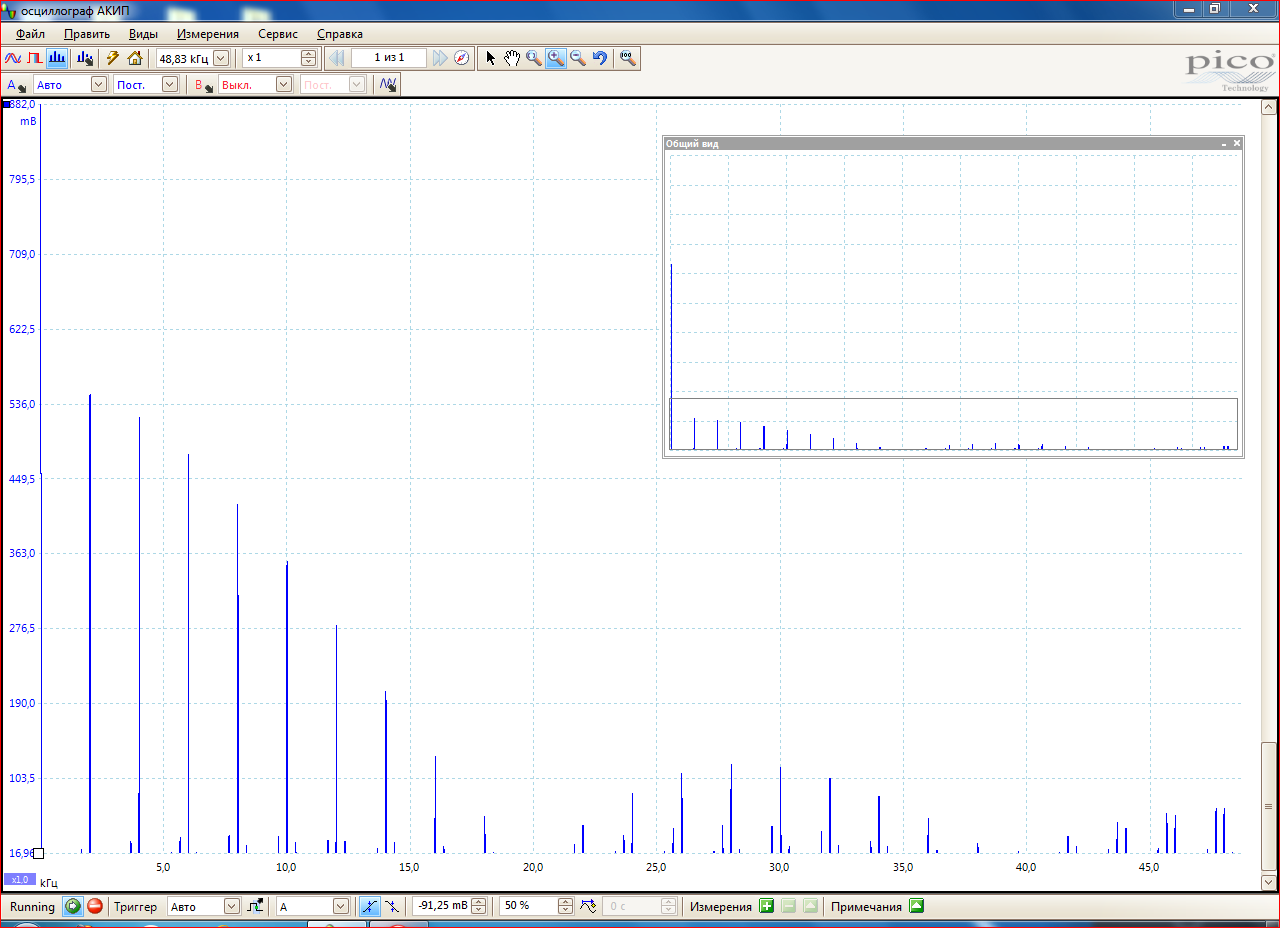
\includegraphics[width=0.95\linewidth]{img/data/A.6/2.0kHz_50us.png}}
                        \caption{Спектр прямоугольного сигнала\\($\nu_{повт} = 2~кГц$; $\tau = 50~мкс$)}
                        \label{plot:A.6.4}
                    \end{minipage}
                \end{figure}

                \begin{figure}[ht]
                    \begin{minipage}[ht]{0.49\linewidth}
                        \center{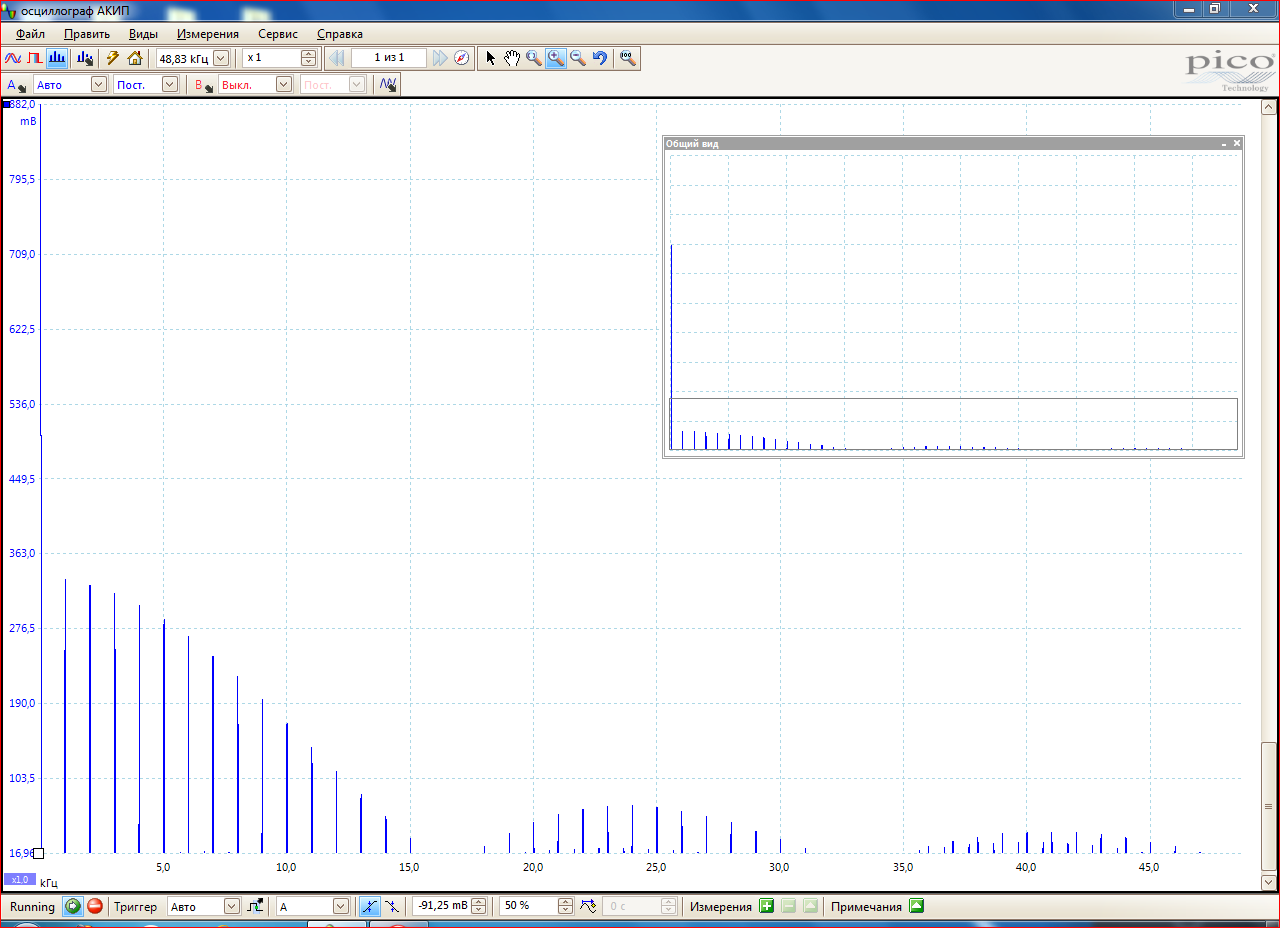
\includegraphics[width=0.95\linewidth]{img/data/A.6/1.0kHz_60us.png}}
                        \caption{Спектр прямоугольного сигнала\\($\nu_{повт} = 1~кГц$; $\tau = 60~мкс$)}
                        \label{plot:A.6.5}
                    \end{minipage}
                    \begin{minipage}[ht]{0.49\linewidth}
                        \center{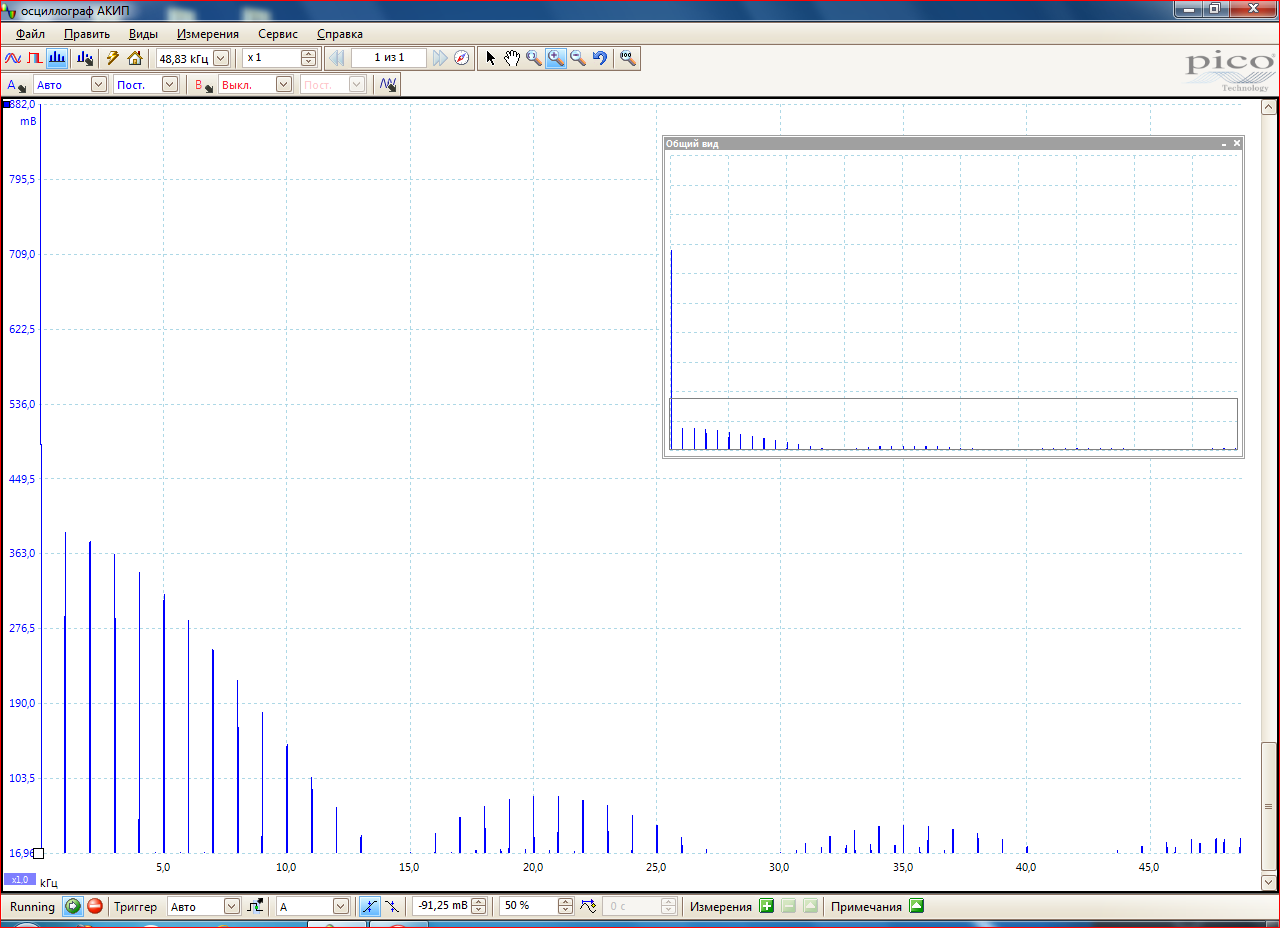
\includegraphics[width=0.95\linewidth]{img/data/A.6/1.0kHz_70us.png}}
                        \caption{Спектр прямоугольного сигнала\\($\nu_{повт} = 1~кГц$; $\tau = 70~мкс$)}
                        \label{plot:A.6.6}
                    \end{minipage}
                \end{figure}

                \begin{figure}[ht]
                    \centering
                    \begin{minipage}[ht]{0.49\linewidth}
                        \center{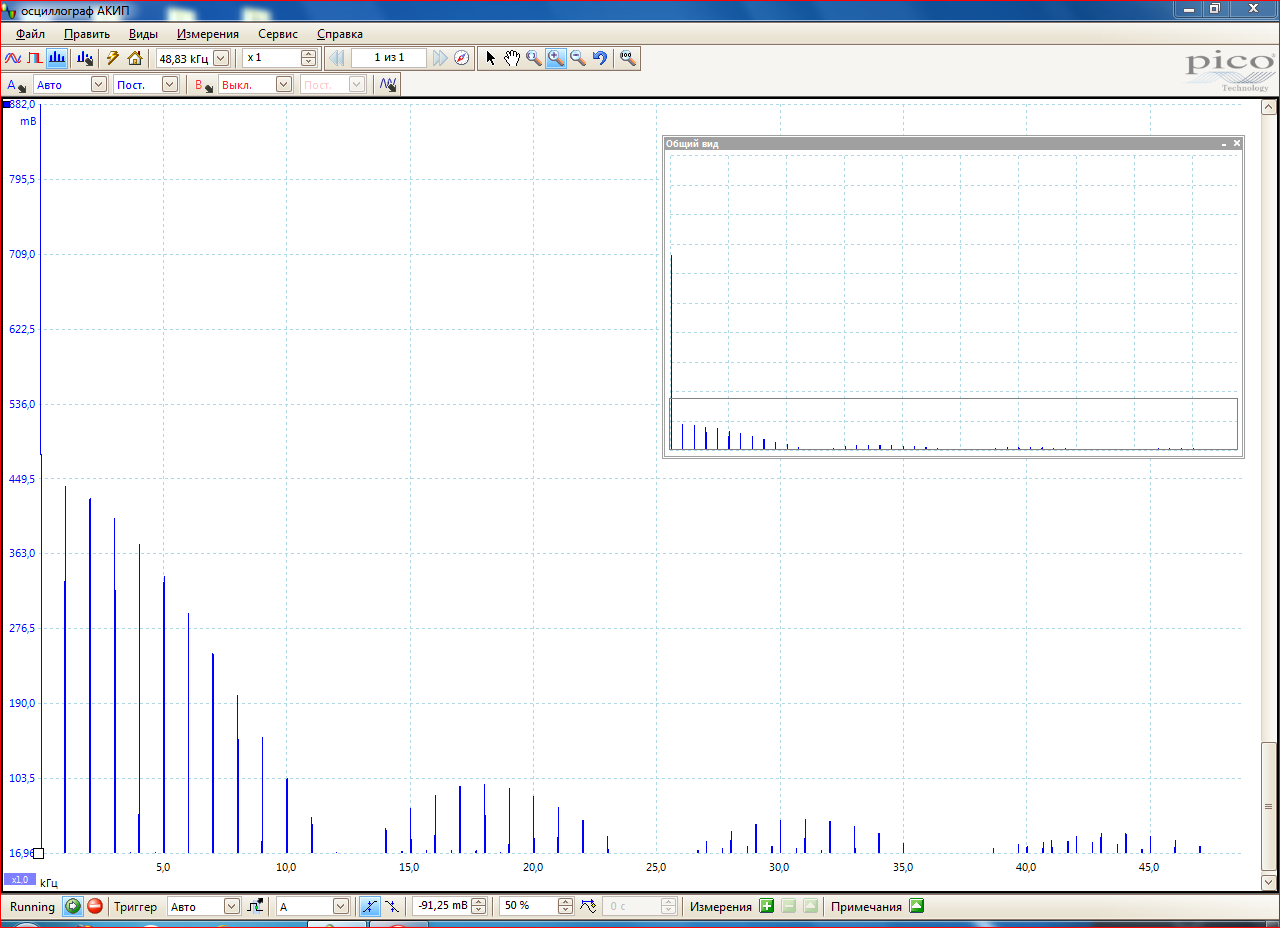
\includegraphics[width=0.95\linewidth]{img/data/A.6/1.0kHz_80us.png}}
                        \caption{Спектр прямоугольного сигнала\\($\nu_{повт} = 1~кГц$; $\tau = 80~мкс$)}
                        \label{plot:A.6.7}
                    \end{minipage}
                \end{figure}

            \subsubsection{Измерение параматров спектра}

                Теоретические формулы:

                \begin{align*}
                    \nu_n^{теор} &= \frac{n}{T}, & \vert a_n \vert &= \frac{\vert sin\frac{\pi n \tau}{T} \vert}{\pi n} = \frac{\tau}{T} \frac{\vert sin \pi \nu_n \tau \vert}{\pi \nu_n \tau}
                \end{align*}

                Результаты измерений и расчётов в таблице \ref{tab:A.7}

                \begin{table}[!ht]
                    \centering
                    \begin{tabular}{|c|c|c|c|c|c|}
                        \hline

                        $n$ & 1 & 2 & 3 & 4 & 5\\ \hline
                        $\nu_n^{эксп}, кГц$ & $1.00 \pm 0.01$ & $2.00 \pm 0.01$ & $3.00 \pm 0.01$ & $4.00 \pm 0.01$ & $5.00 \pm 0.01$\\ \hline
                        $\nu_n^{теор}, кГц$ & 1 & 2 & 3 & 4 & 5\\ \hline
                        $\vert a_n \vert^{эксп}, усл. ед.$ & $279.0 \pm 1.0$ & $274.0 \pm 1.0$ & $269.0 \pm 1.0$ & $261.0 \pm 1.0$ & $251.0 \pm 1.0$\\ \hline
                        $\vert a_n/a_1 \vert^{эксп}$ & $1.000 \pm 0.005$ & $0.982 \pm 0.005$ & $0.964 \pm 0.005$ & $0.935 \pm 0.005$ & $0.900 \pm 0.005$\\ \hline
                        $\vert a_n/a_1 \vert^{теор}$ & 1 & 0.987688 & 0.967371 & 0.939347 & 0.904029\\ \hline

                    \end{tabular}
                    \begin{tabular}{|c|c|c|c|}
                        \hline

                        $n$ & 6 & 7 & 8\\ \hline
                        $\nu_n^{эксп}, кГц$ & $6.00 \pm 0.01$ & $7.00 \pm 0.01$ & $8.00 \pm 0.01$\\ \hline
                        $\nu_n^{теор}, кГц$ & 6 & 7 & 8\\ \hline
                        $\vert a_n \vert^{эксп}, усл. ед.$ & $239.0 \pm 1.0$ & $226.0 \pm 1.0$ & $211.0 \pm 1.0$\\ \hline
                        $\vert a_n/a_1 \vert^{эксп}$ & $0.857 \pm 0.005$ & $0.810 \pm 0.005$ & $0.756 \pm 0.004$\\ \hline
                        $\vert a_n/a_1 \vert^{теор}$ & 0.861934 & 0.813674 & 0.759948\\ \hline

                    \end{tabular}
                    \caption{Параметры спектра прямоугольного сигнала}
                    \label{tab:A.7}
                \end{table}

            \subsubsection{Измерение полной ширины спектра при различных длинах импульса}

                Зафиксируем $T = 1~мс$. Результаты в таблице \ref{tab:A.8}

                \begin{table}[ht]
                    \begin{minipage}[ht]{0.49\linewidth}
                        \centering
                        \begin{tabular}{|c|c|}
                            \hline

                            $\tau, мкс$ & $\Delta \nu, кГц$\\ \hline
                            20 & $52.0 \pm 0.5$\\ \hline
                            30 & $33.0 \pm 0.5$\\ \hline
                            40 & $25.0 \pm 0.5$\\ \hline
                            50 & $20.0 \pm 0.5$\\ \hline
                            60 & $16.0 \pm 0.5$\\ \hline
                            70 & $14.0 \pm 0.5$\\ \hline
                            80 & $13.0 \pm 0.5$\\ \hline
                            90 & $11.0 \pm 0.5$\\ \hline
                            100 & $10.0 \pm 0.5$\\ \hline
                            110 & $9.0 \pm 0.5$\\ \hline
                            120 & $8.0 \pm 0.5$\\ \hline
                            130 & $8.0 \pm 0.5$\\ \hline
                            140 & $7.0 \pm 0.5$\\ \hline
                            150 & $6.0 \pm 0.5$\\ \hline
                            160 & $6.0 \pm 0.5$\\ \hline
                            170 & $6.0 \pm 0.5$\\ \hline
                            180 & $6.0 \pm 0.5$\\ \hline
                            190 & $5.0 \pm 0.5$\\ \hline
                            200 & $5.0 \pm 0.5$\\ \hline

                        \end{tabular}
                        \caption{Зависимость полной ширины спектра от длительности импульса}
                        \label{tab:A.8}
                    \end{minipage}
                    \begin{minipage}[ht]{0.49\linewidth}
                        \centering
                        \begin{tabular}{|c|c|}
                            \hline

                            $T, мкс$ & $\delta \nu, кГц$\\ \hline
                            200 & $5.13 \pm 0.01$\\ \hline
                            600 & $1.67 \pm 0.01$\\ \hline
                            1000 & $1.00 \pm 0.01$\\ \hline
                            1400 & $0.70 \pm 0.01$\\ \hline
                            1800 & $0.55 \pm 0.01$\\ \hline
                            2200 & $0.46 \pm 0.01$\\ \hline
                            2600 & $0.39 \pm 0.01$\\ \hline
                            3000 & $0.34 \pm 0.01$\\ \hline
                            3400 & $0.29 \pm 0.01$\\ \hline
                            3800 & $0.27 \pm 0.01$\\ \hline
                            4200 & $0.24 \pm 0.01$\\ \hline
                            4600 & $0.22 \pm 0.01$\\ \hline
                            5000 & $0.20 \pm 0.01$\\ \hline

                        \end{tabular}
                        \caption{Зависимость расстояния между соседними гармониками от периода повторения}
                        \label{tab:A.9}
                    \end{minipage}
                \end{table}

            \subsubsection{Измерение расстояния между соседними гармониками при различных периодах повторения сигнала}

                Зафиксируем $\tau = 100~мкс$. Результаты в таблице \ref{tab:A.9}

            \subsubsection{Графики зависимостей $\Delta \nu(1/\tau)$ и $\delta \nu(1/T)$. Проверка соотношений неопределённости}

                Графики на рисунках \ref{plot:A.10.1} и \ref{plot:A.10.2}

                Проверим соотношения неопределённостей: $\Delta \nu \sim \frac{1}{\tau}$ и $\delta \nu \sim \frac{1}{T}$

                По МНК коэффициенты: $k_{\tau} = 1.012 \pm 0.007$; $k_{T} = 1.021 \pm 0.003$. Как видим соотношения выполняются с хорошей точностью.

                \begin{figure}[ht]
                    \begin{minipage}[ht]{0.49\linewidth}
                        \center{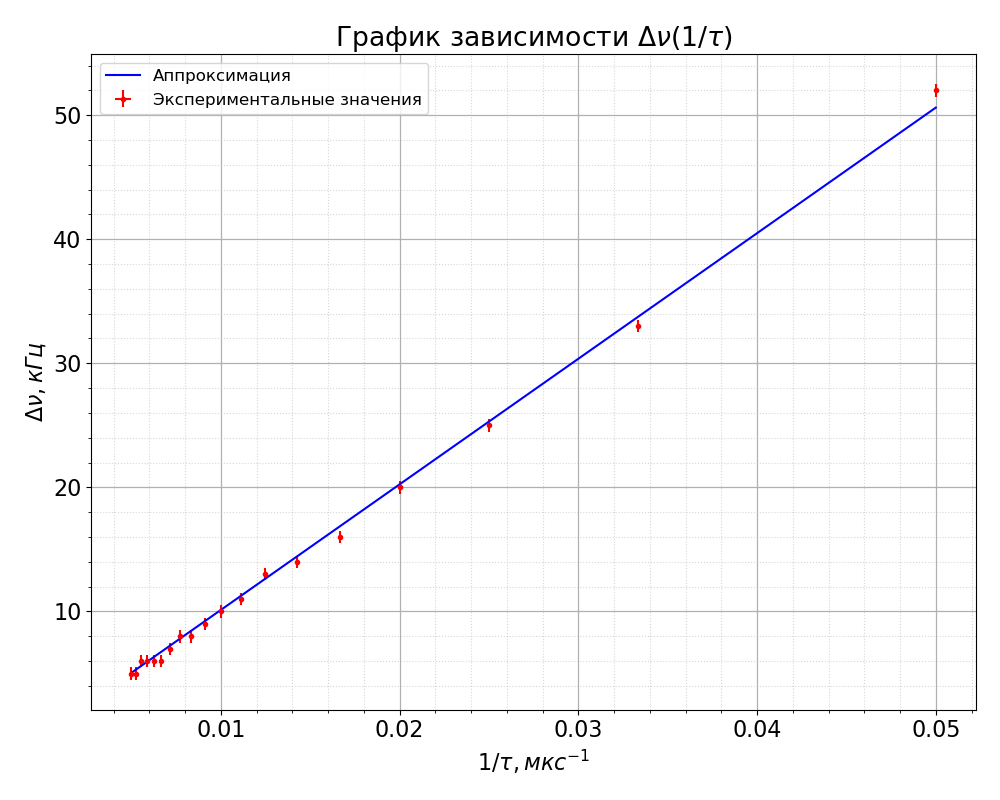
\includegraphics[width=0.95\linewidth]{img/plot_A.10.1.png}}
                        \caption{График зависимости $\Delta \nu(1/\tau)$}
                        \label{plot:A.10.1}
                    \end{minipage}
                    \begin{minipage}[ht]{0.49\linewidth}
                        \center{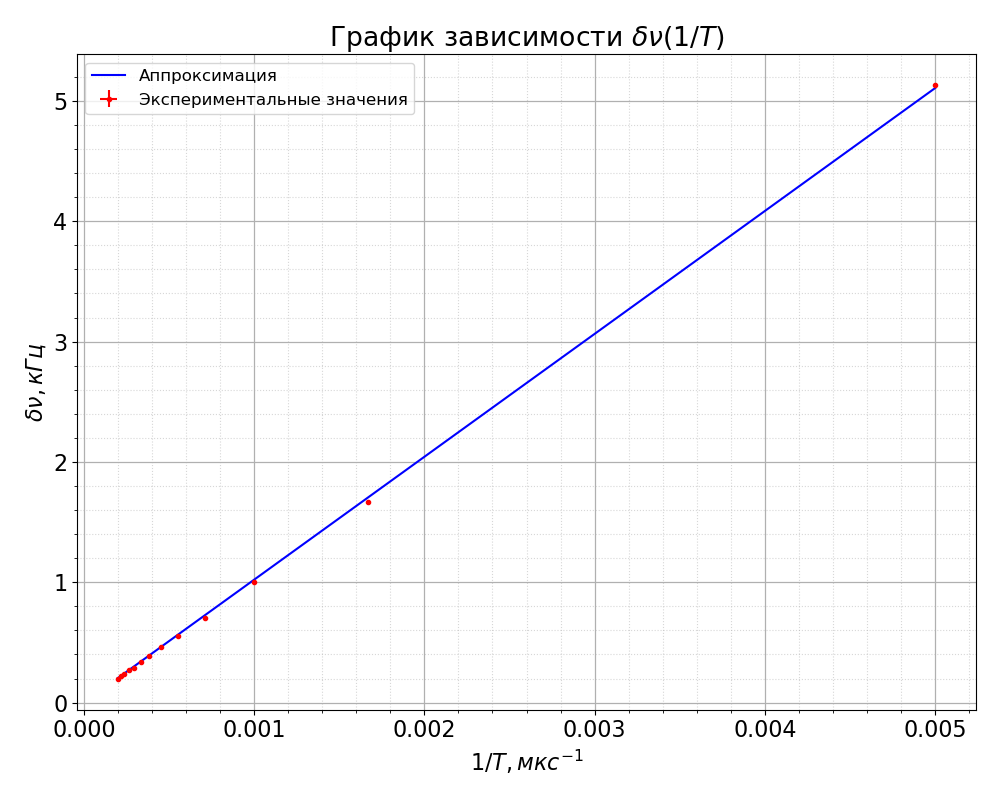
\includegraphics[width=0.95\linewidth]{img/plot_A.10.2.png}}
                        \caption{График зависимости $\delta \nu(1/T)$}
                        \label{plot:A.10.2}
                    \end{minipage}
                \end{figure}

        \subsection{Наблюдение периодической последовательности цугов}
            \setcounter{subsubsection}{10}
            \subsubsection{Устойчивая картина цугов на экране осциллографа}

                Частота несущей $\nu_0 = 50~кГц$, период повторения $T = 1~мс$, число периодов синусоиды в одном импульсе $N = 5$

                Получили картину на рисунке \ref{plot:B.11}

                \begin{figure}[ht]
                    \centering
                    \begin{minipage}[ht]{0.49\linewidth}
                        \center{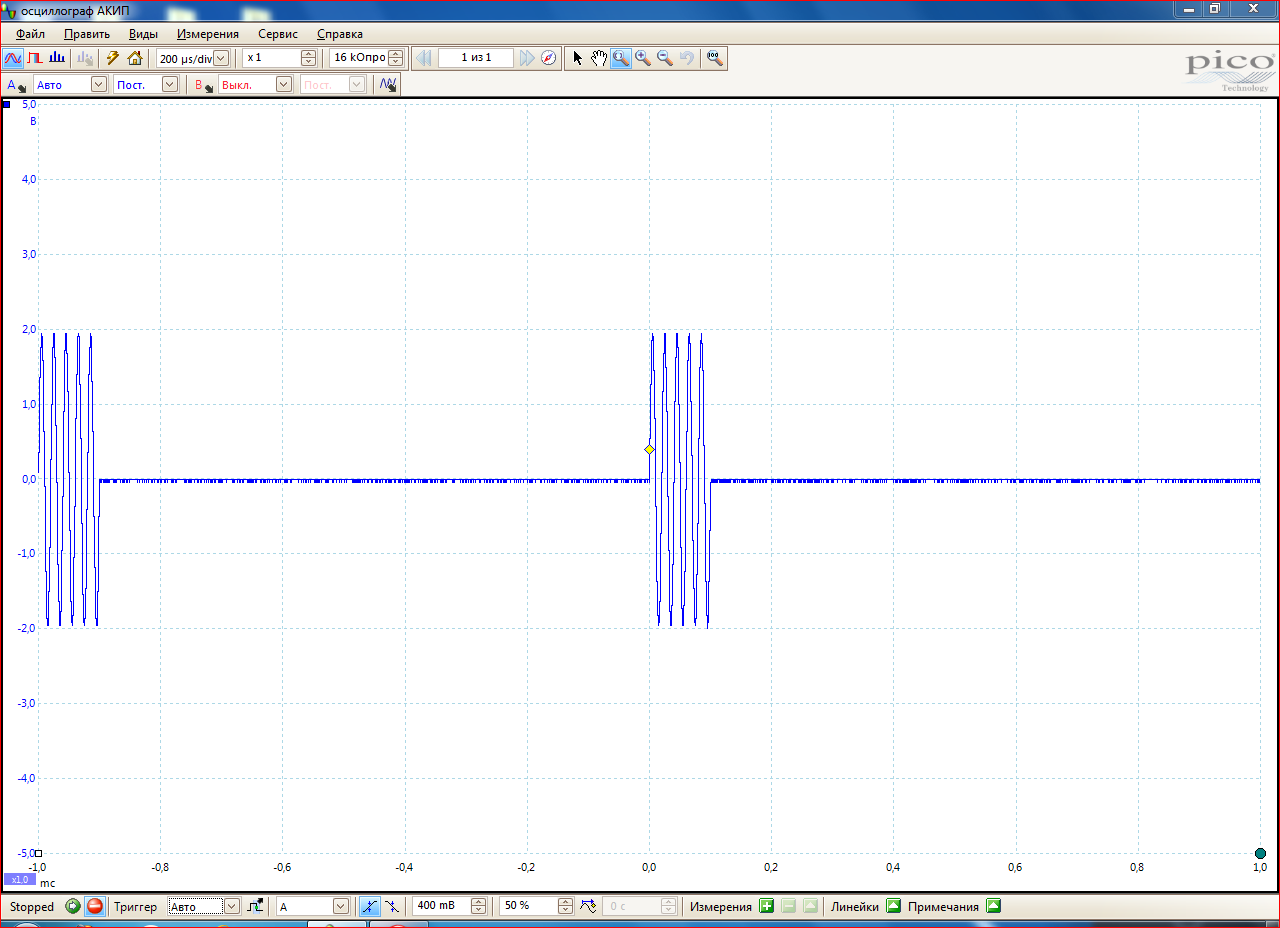
\includegraphics[width=0.95\linewidth]{img/data/B.11.png}}
                        \caption{Устойчивая картина цугов}
                        \label{plot:B.11}
                    \end{minipage}
                \end{figure}

            \subsubsection{Спектр периодической последовательности цугов}

                Спектр для сигнала с теми же параметрами на рисунке \ref{plot:B.13.1}

            \subsubsection{Изменение спектра при изменении параметров}

                Спектры представлены на рисунках \ref{plot:B.13.1}, \ref{plot:B.13.2}, \ref{plot:B.13.3} и \ref{plot:B.13.4}

                \begin{figure}[ht]
                    \begin{minipage}[ht]{0.49\linewidth}
                        \center{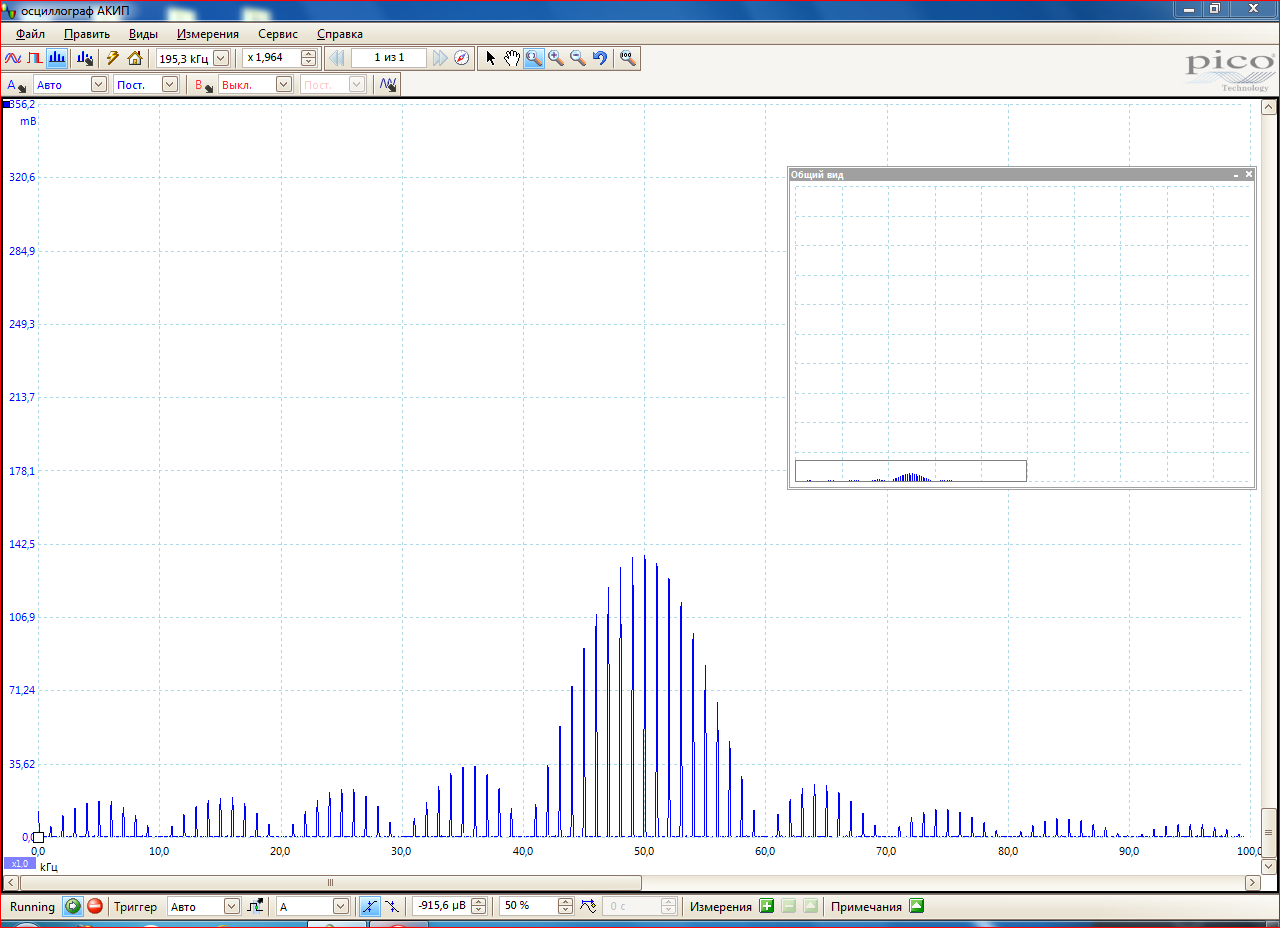
\includegraphics[width=0.95\linewidth]{img/data/B.13/50kHz_1ms_5.png}}
                        \caption{Спектр цугов\\($\nu_0 = 50~кГц$; $T = 1~мс$; $N = 5$)}
                        \label{plot:B.13.1}
                    \end{minipage}
                    \begin{minipage}[ht]{0.49\linewidth}
                        \center{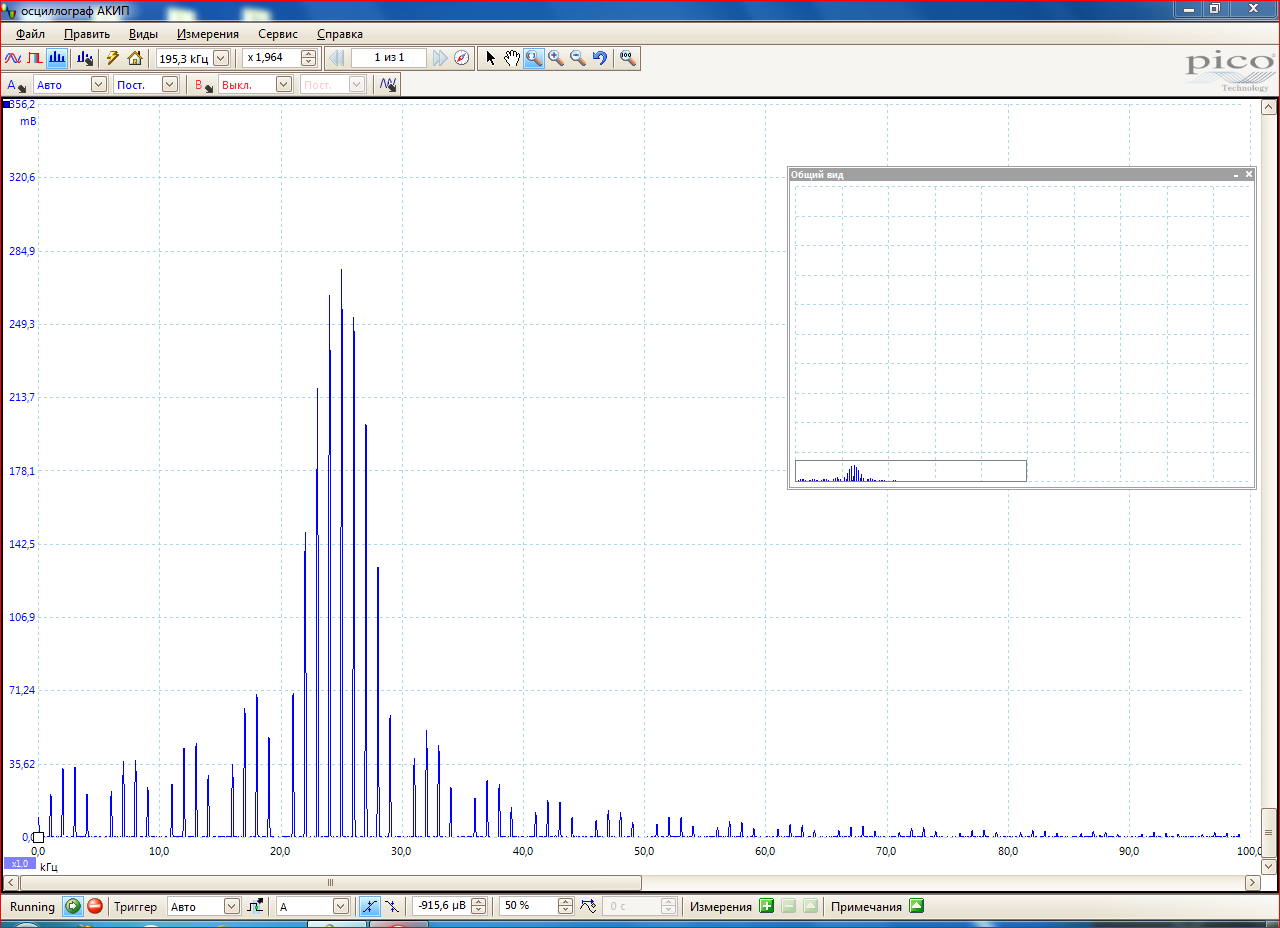
\includegraphics[width=0.95\linewidth]{img/data/B.13/25kHz_1ms_5.png}}
                        \caption{Спектр цугов\\($\nu_0 = 25~кГц$; $T = 1~мс$; $N = 5$)}
                        \label{plot:B.13.2}
                    \end{minipage}
                \end{figure}

                \begin{figure}[ht]
                    \begin{minipage}[ht]{0.49\linewidth}
                        \center{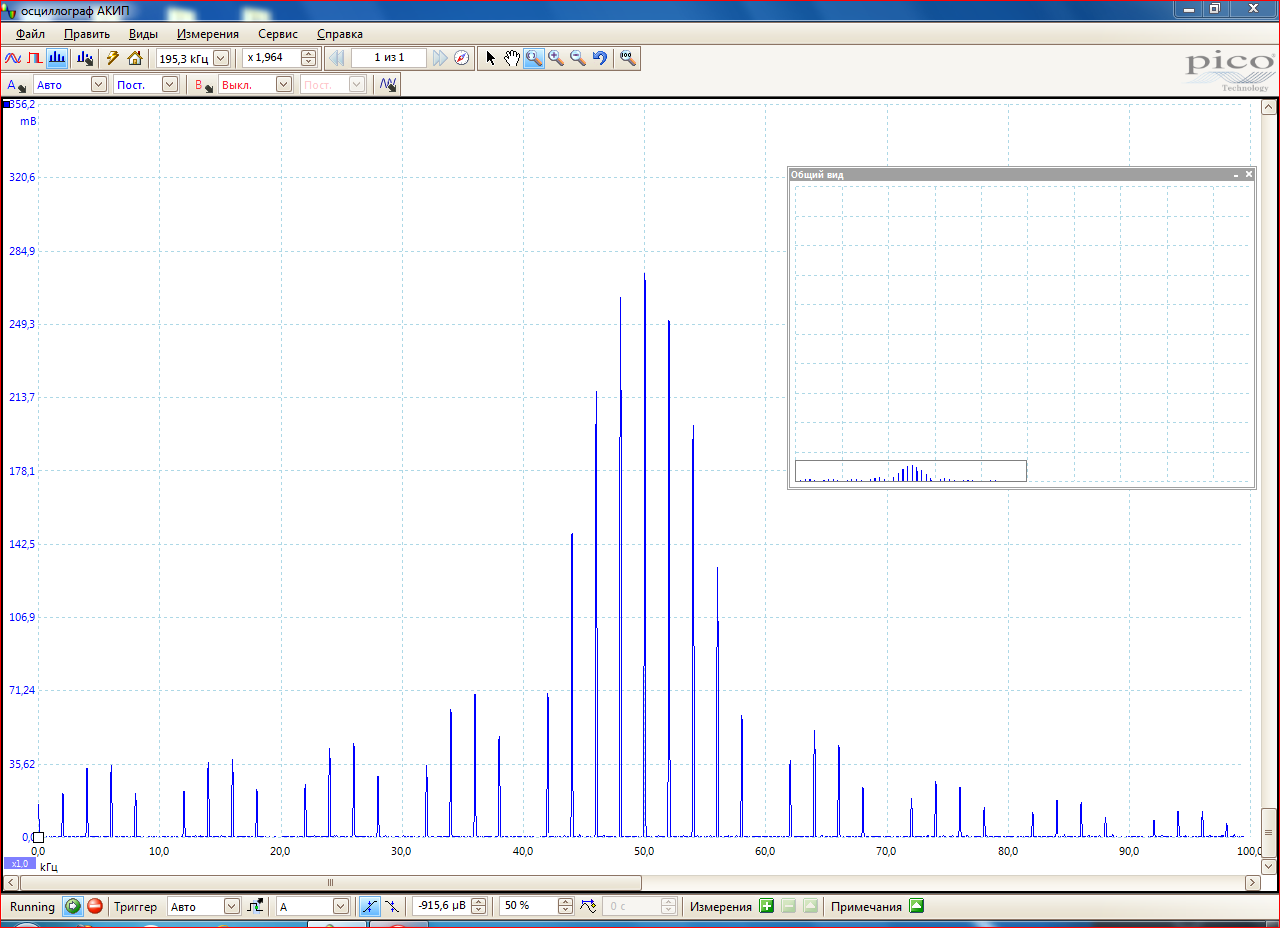
\includegraphics[width=0.95\linewidth]{img/data/B.13/50kHz_0.5ms_5.png}}
                        \caption{Спектр цугов\\($\nu_0 = 50~кГц$; $T = 0.5~мс$; $N = 5$)}
                        \label{plot:B.13.3}
                    \end{minipage}
                    \begin{minipage}[ht]{0.49\linewidth}
                        \center{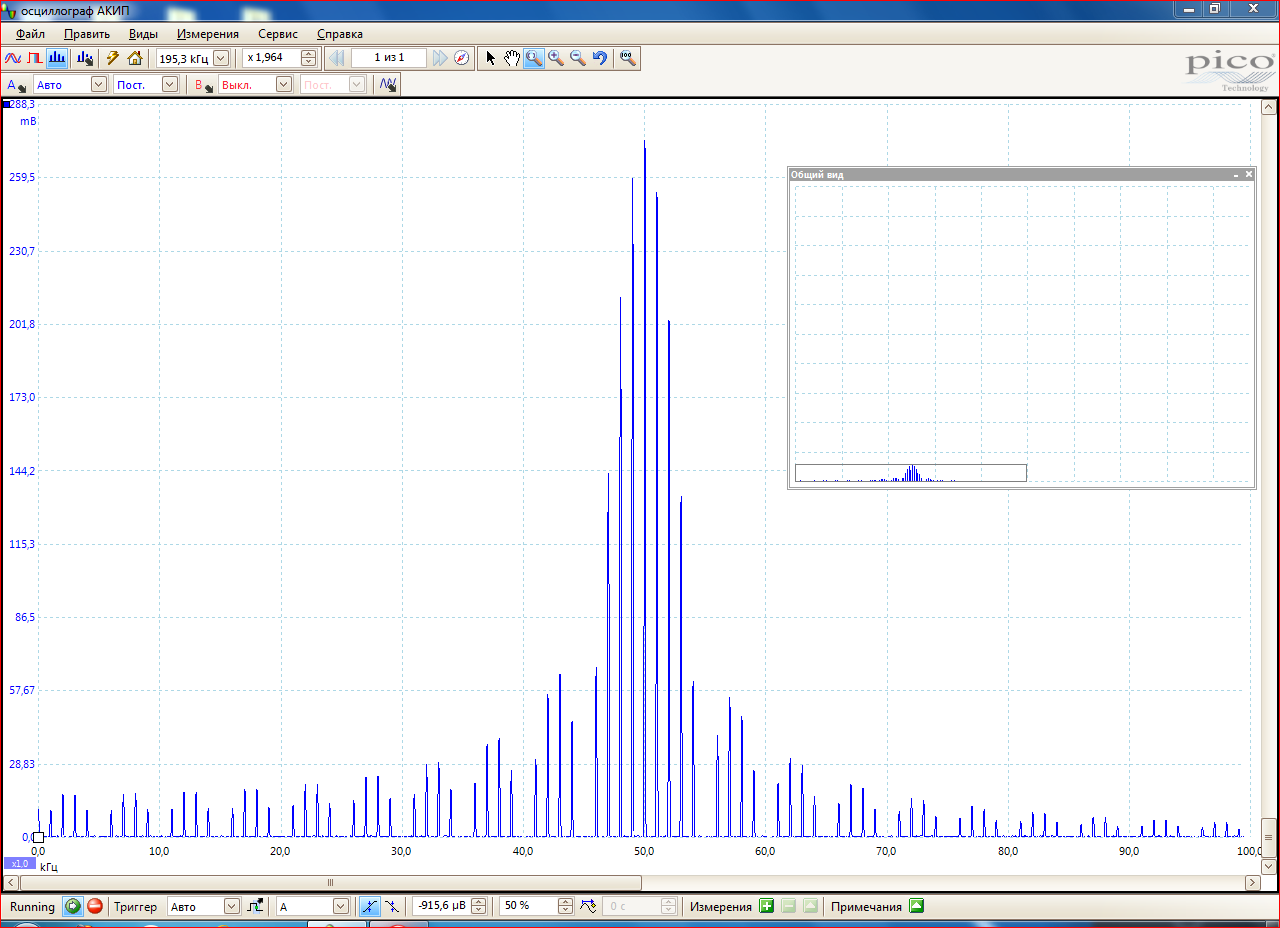
\includegraphics[width=0.95\linewidth]{img/data/B.13/50kHz_1ms_10.png}}
                        \caption{Спектр цугов\\($\nu_0 = 50~кГц$; $T = 1~мс$; $N = 10$)}
                        \label{plot:B.13.4}
                    \end{minipage}
                \end{figure}

            \subsubsection{Параметры спектров, проверка соотношений неопределённостей}

                Проверим соотношения неопределённостей: должно выполняться $\Delta \nu \cdot \tau_0 \sim 1$ и $\delta \nu \cdot T \sim 1$

                По теореме смещения, смещение по времени не меняет амплитуд спектральных компонент, а лишь сдвигает их фазы (пропорционально частоте компоненты)

                \begin{table}[!ht]
                    \centering
                    \begin{tabular}{|c|c|c|c|c|c|}
                        \hline

                        $\tau_0, мс$ & $\Delta \nu, кГц$ & $\Delta \nu \cdot \tau_0$ & $T, мс$ & $\delta \nu, кГц$ & $\delta \nu \cdot T$\\ \hline
                        0.02 & 10 & 0.2 & 1 & 1 & 1\\ \hline
                        0.04 & 5 & 0.2 & 1 & 1 & 1\\ \hline
                        0.02 & 10 & 0.2 & 0.5 & 2 & 1\\ \hline
                        0.02 & 5 & 0.1 & 1 & 1 & 1\\ \hline

                    \end{tabular}
                    \caption{Параметры спектра последовательности цугов}
                    \label{tab:B.14}
                \end{table}

        \setcounter{subsection}{3}
        \subsection{Исследование спектра амплитудно-модулированного сигнала}

            \setcounter{subsubsection}{18}
            \subsubsection{Модулированный по амплитуде синусоидальный сигнал}

                Частота несущей $\nu_0 = 50~кГц$, частота модуляции $\nu_{мод} = 2~кГц$, глубина модуляции $50~\% (m = 0.5)$

                Устойчивая картина сигнала на рисунке \ref{plot:D.19}

                \begin{figure}[ht]
                    \centering
                    \begin{minipage}[ht]{0.49\linewidth}
                        \center{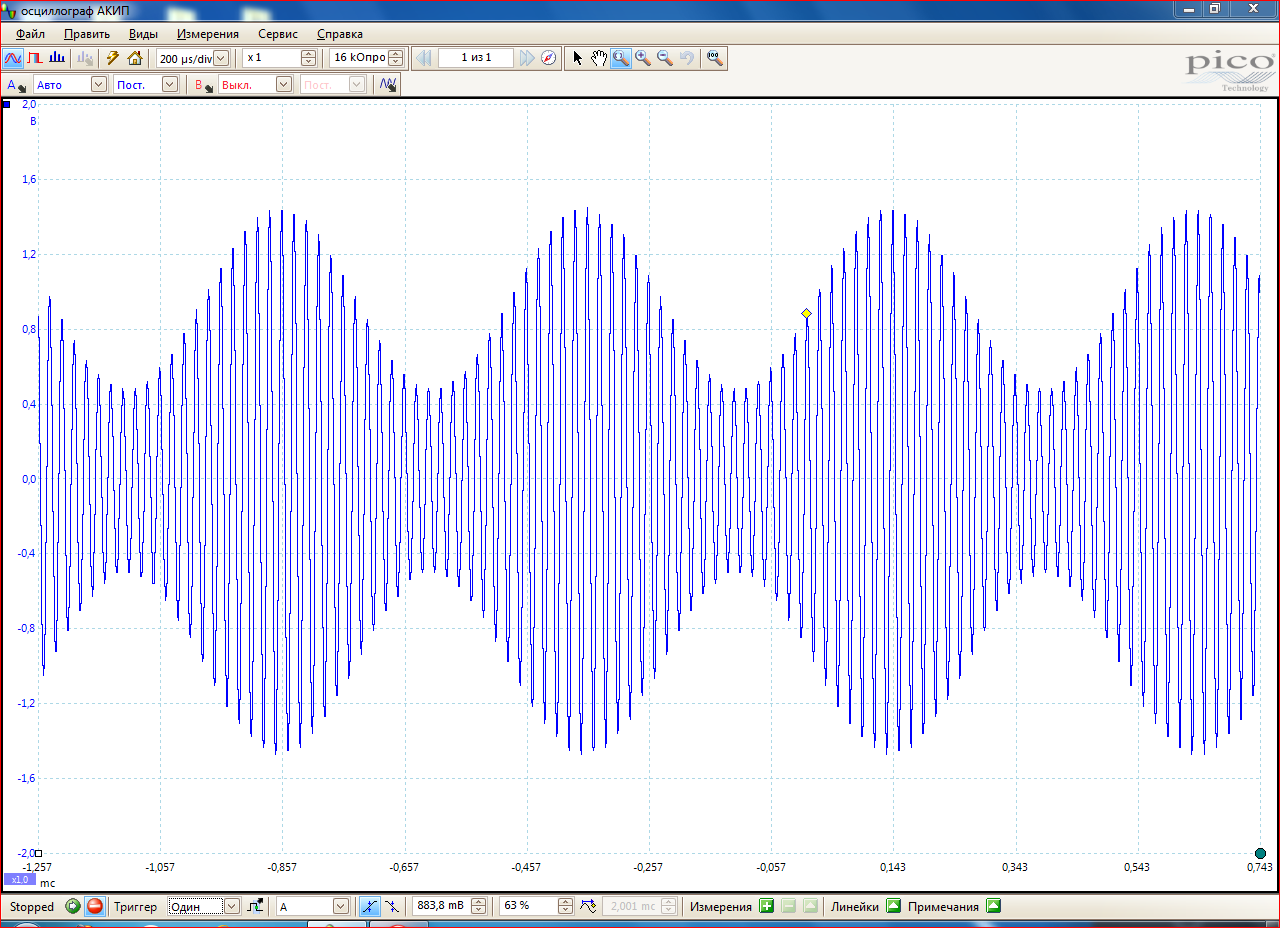
\includegraphics[width=0.95\linewidth]{img/data/D.19.png}}
                        \caption{Устойчивая картина модулированного сигнала}
                        \label{plot:D.19}
                    \end{minipage}
                \end{figure}

            \subsubsection{Параметры сигнала}

                \begin{align*}
                    A_{max} &= 1.44~В & A_{min} &= 0.48~В
                \end{align*}

                $$
                    m = \frac{A_{max} - A_{min}}{A_{max} + A_{min}} = \frac{1.44 - 0.48}{1.44 + 0.48} = 0.5 = 50\%
                $$

                Равенство выполняется

            \subsubsection{Спектр сигнала}

                Спектры сигнала при различных параметров на рисунках \ref{plot:D.21.1}, \ref{plot:D.21.2}, \ref{plot:D.21.3} и \ref{plot:D.21.4}

                Параметры в таблице \ref{tab:D.21}

                \begin{figure}[ht]
                    \begin{minipage}[ht]{0.49\linewidth}
                        \center{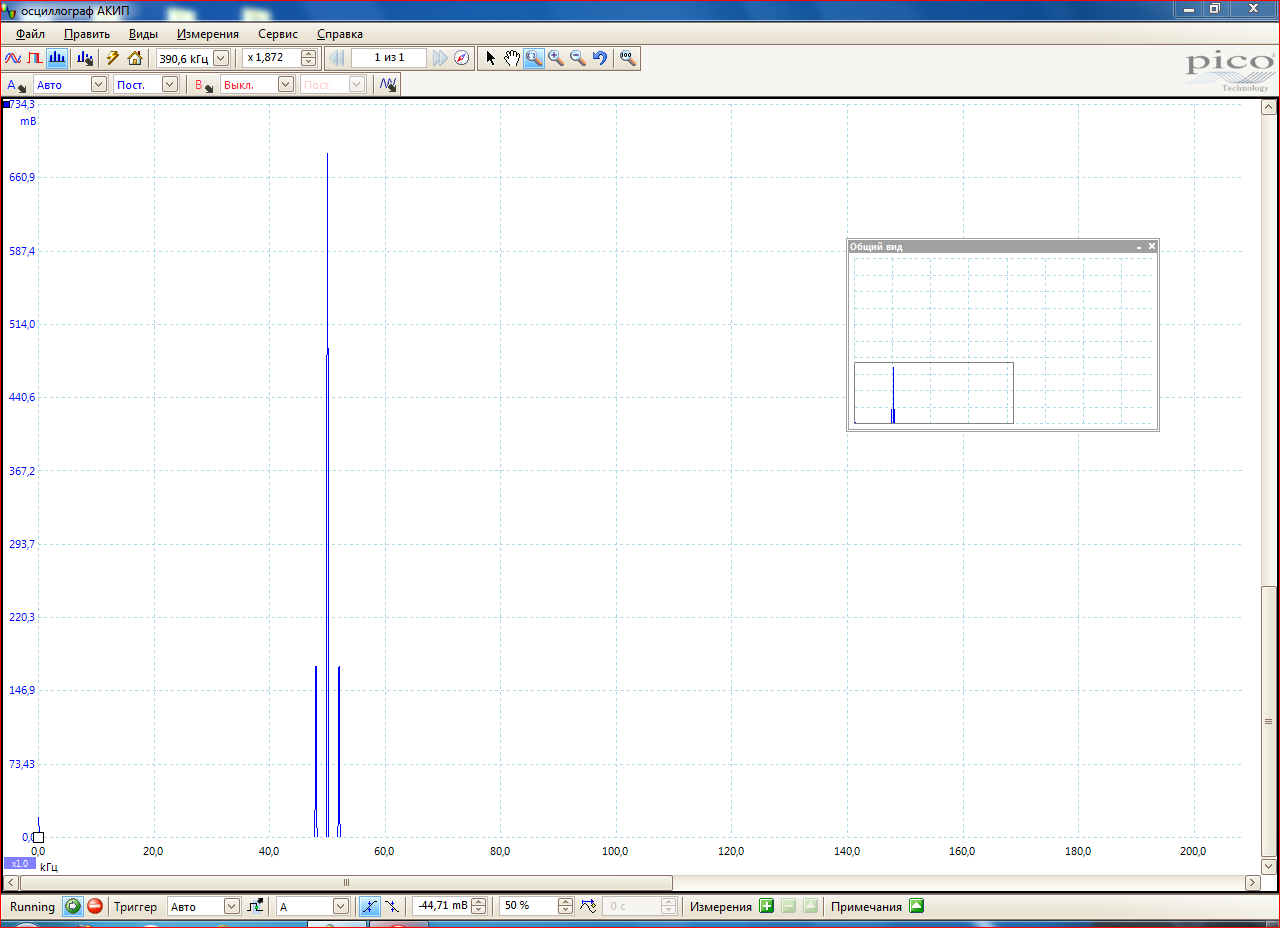
\includegraphics[width=0.95\linewidth]{img/data/D.21/50kHz_2kHz_0.5.png}}
                        \caption{Спектр модулированного сигнала\\($\nu_0 = 50~кГц$; $\nu_{мод} = 2~кГц$; $m = 0.5$)}
                        \label{plot:D.21.1}
                    \end{minipage}
                    \begin{minipage}[ht]{0.49\linewidth}
                        \center{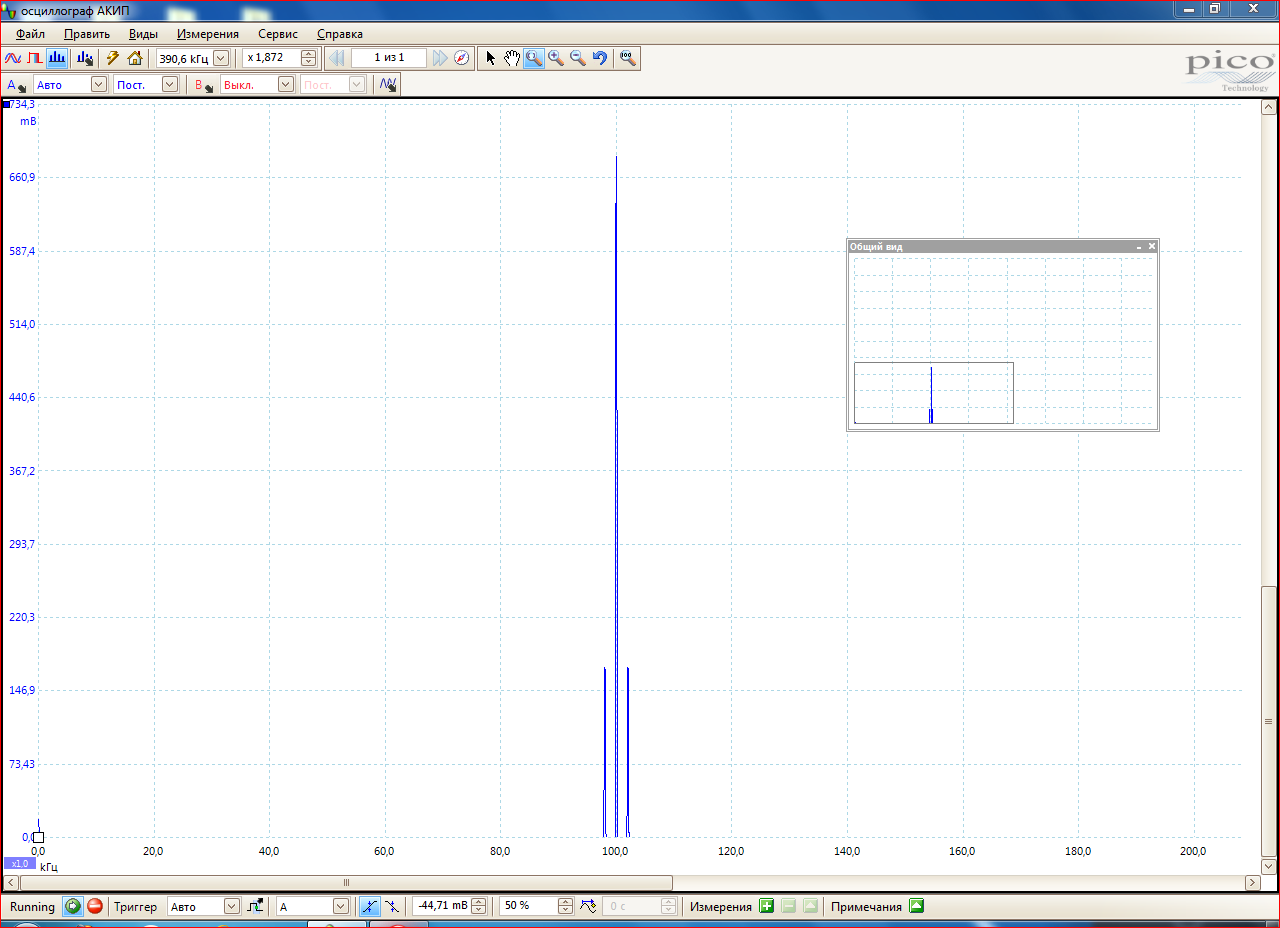
\includegraphics[width=0.95\linewidth]{img/data/D.21/100kHz_2kHz_0.5.png}}
                        \caption{Спектр модулированного сигнала\\($\nu_0 = 100~кГц$; $\nu_{мод} = 2~кГц$; $m = 0.5$)}
                        \label{plot:D.21.2}
                    \end{minipage}
                \end{figure}

                \begin{figure}[ht]
                    \begin{minipage}[ht]{0.49\linewidth}
                        \center{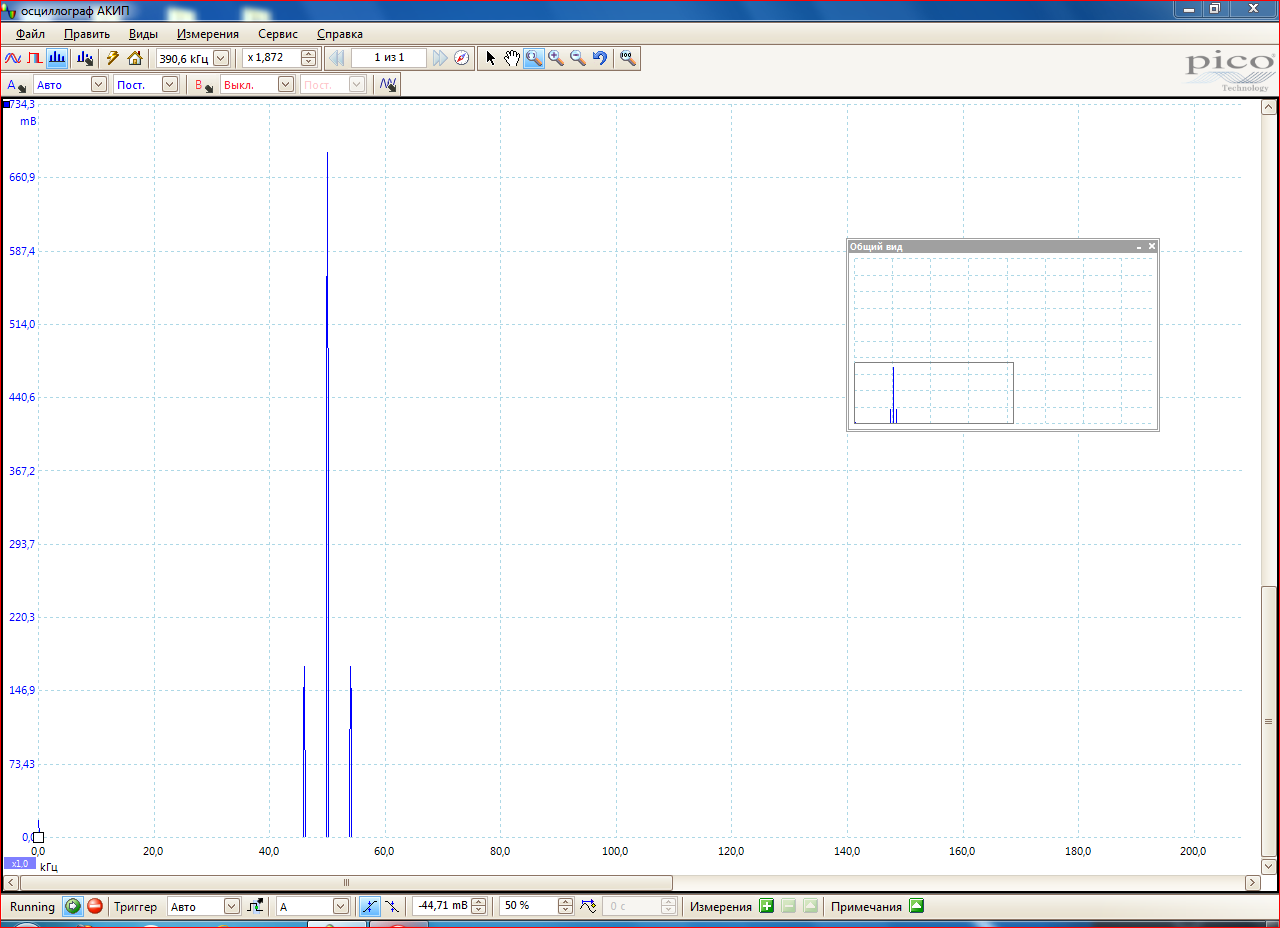
\includegraphics[width=0.95\linewidth]{img/data/D.21/50kHz_4kHz_0.5.png}}
                        \caption{Спектр модулированного сигнала\\($\nu_0 = 50~кГц$; $\nu_{мод} = 4~кГц$; $m = 0.5$)}
                        \label{plot:D.21.3}
                    \end{minipage}
                    \begin{minipage}[ht]{0.49\linewidth}
                        \center{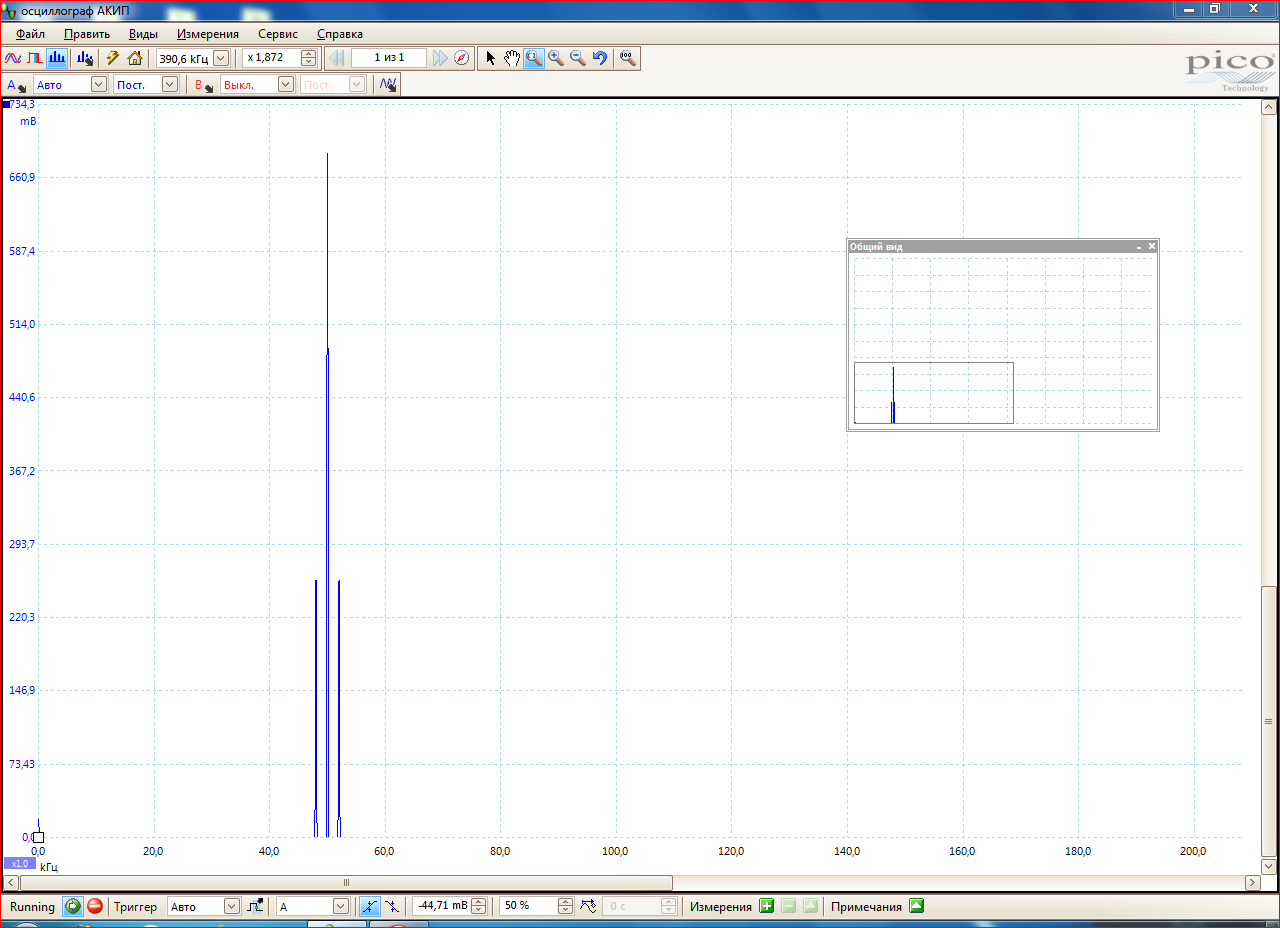
\includegraphics[width=0.95\linewidth]{img/data/D.21/50kHz_2kHz_0.75.png}}
                        \caption{Спектр модулированного сигнала\\($\nu_0 = 50~кГц$; $\nu_{мод} = 2~кГц$; $m = 0.75$)}
                        \label{plot:D.21.4}
                    \end{minipage}
                \end{figure}

                \begin{table}[!ht]
                    \centering
                    \begin{tabular}{|c|c|c|c|c|}
                        \hline

                        $\nu_0, кГц$ & $\nu_{мод}, кГц$ & m & $\nu_0^{изм}, кГц$ & $\nu_{мод}^{изм}, кГц$\\ \hline
                        50 & 2 & 0.5 & 50 & 2\\ \hline
                        100 & 2 & 0.5 & 100 & 2\\ \hline
                        50 & 4 & 0.5 & 50 & 4\\ \hline
                        50 & 2 & 0.75 & 50 & 2\\ \hline

                    \end{tabular}
                    \caption{Параметры спектра модулированного сигнала}
                    \label{tab:D.21}
                \end{table}

            \subsubsection{Отношение амплитуд при различной глубине модуляции}

                Результат в таблице \ref{tab:D.22}

                \begin{table}[!ht]
                    \centering
                    \begin{tabular}{|c|c|c|c|c|c|c|c|c|c|c|}
                        \hline

                        $m, \%$ & 10 & 20 & 30 & 40 & 50 & 60 & 70 & 80 & 90 & 100\\ \hline
                        $\frac{a_{бок}}{a_{осн}}$ & 0.051 & 0.1 & 0.15 & 0.2 & 0.249 & 0.299 & 0.348 & 0.399 & 0.449 & 0.495\\ \hline

                    \end{tabular}
                    \caption{Отношение амплитуд при различной глубине модуляции}
                    \label{tab:D.22}
                \end{table}

            \subsubsection{График зависимости $a_{бок}/a_{осн}$ от $m$}

                Амплитуда боковой гармоники $a_1 = ma_0/2$, где $a_0$ - амплитуда основной гармоники

                График на рисунке \ref{plot:D.23}

                \begin{figure}[ht]
                    \centering
                    \begin{minipage}[ht]{0.49\linewidth}
                        \center{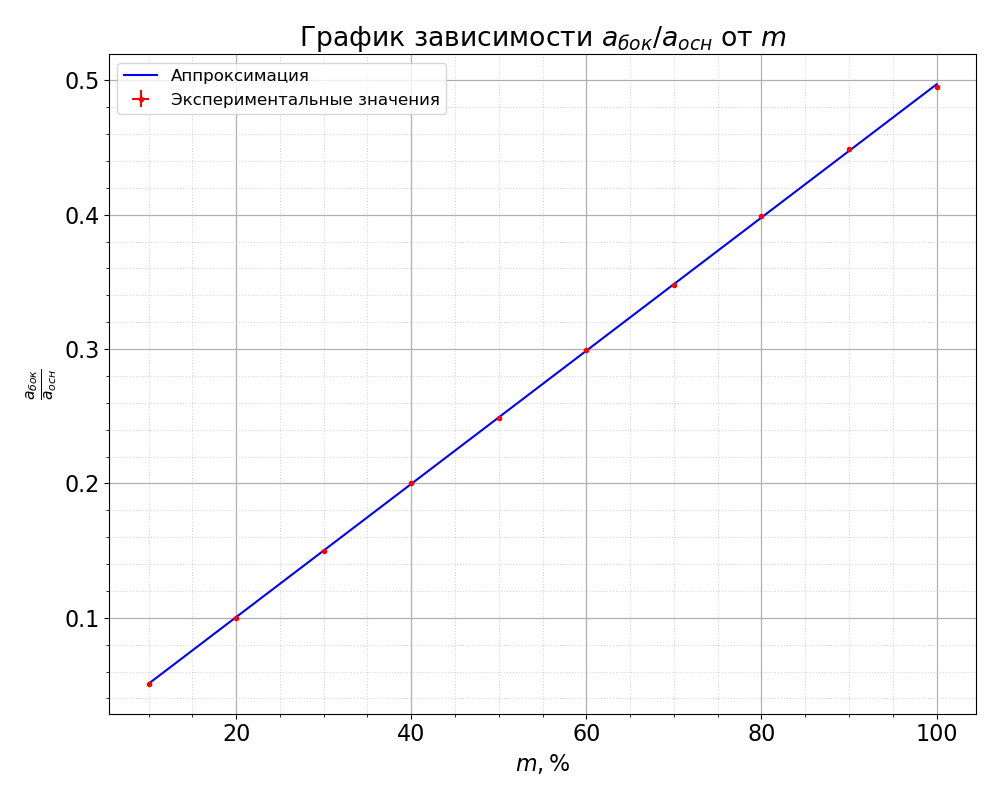
\includegraphics[width=0.95\linewidth]{img/plot_D.23.png}}
                        \caption{График зависимости $a_{бок}/a_{осн}$ от $m$}
                        \label{plot:D.23}
                    \end{minipage}
                \end{figure}

        \setcounter{subsection}{5}
        \subsection{Изучение фильтрации сигналов}

            \setcounter{subsubsection}{23}
            \subsubsection{Параметры RC-цепочки}

                \begin{align*}
                    R &= 3~кОм & C &= 1000~пФ & \tau_{RC} &= RC = 3~мкс & \nu_{RC} &= 1/\nu_{RC} = 0.33~МГц
                \end{align*}

                Подадим последовательность прямоугольных импульсов с периодом повторения $T = 3~мкс \sim \tau_{RC}$ и длительностью $\tau = 150~нс \sim T/20$

            \subsubsection{Сигналы и спектры при различных значениях $T$}

                Сигналы на рисунках \ref{plot:F.27.1}, \ref{plot:F.27.2} и \ref{plot:F.27.3}

                Спектры на рисунках \ref{plot:F.27.4}, \ref{plot:F.27.5} и \ref{plot:F.27.6}

                \begin{figure}[ht]
                    \begin{minipage}[ht]{0.49\linewidth}
                        \center{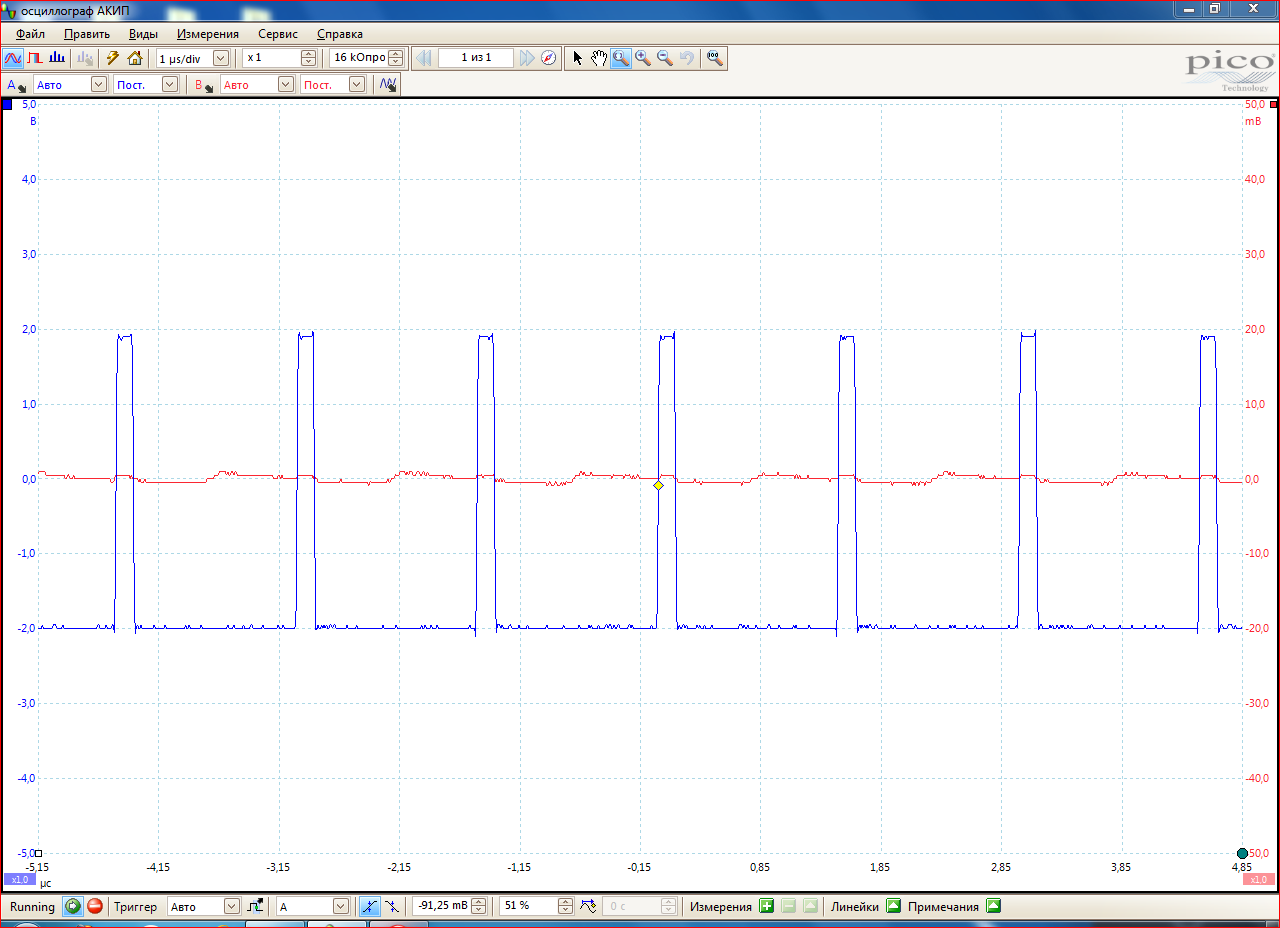
\includegraphics[width=0.95\linewidth]{img/data/F.27/1.5us_150ns.png}}
                        \caption{Прямоугольные импульсы\\($T = 1.5~мкс$; $\tau = 150~нс$)}
                        \label{plot:F.27.1}
                    \end{minipage}
                    \begin{minipage}[ht]{0.49\linewidth}
                        \center{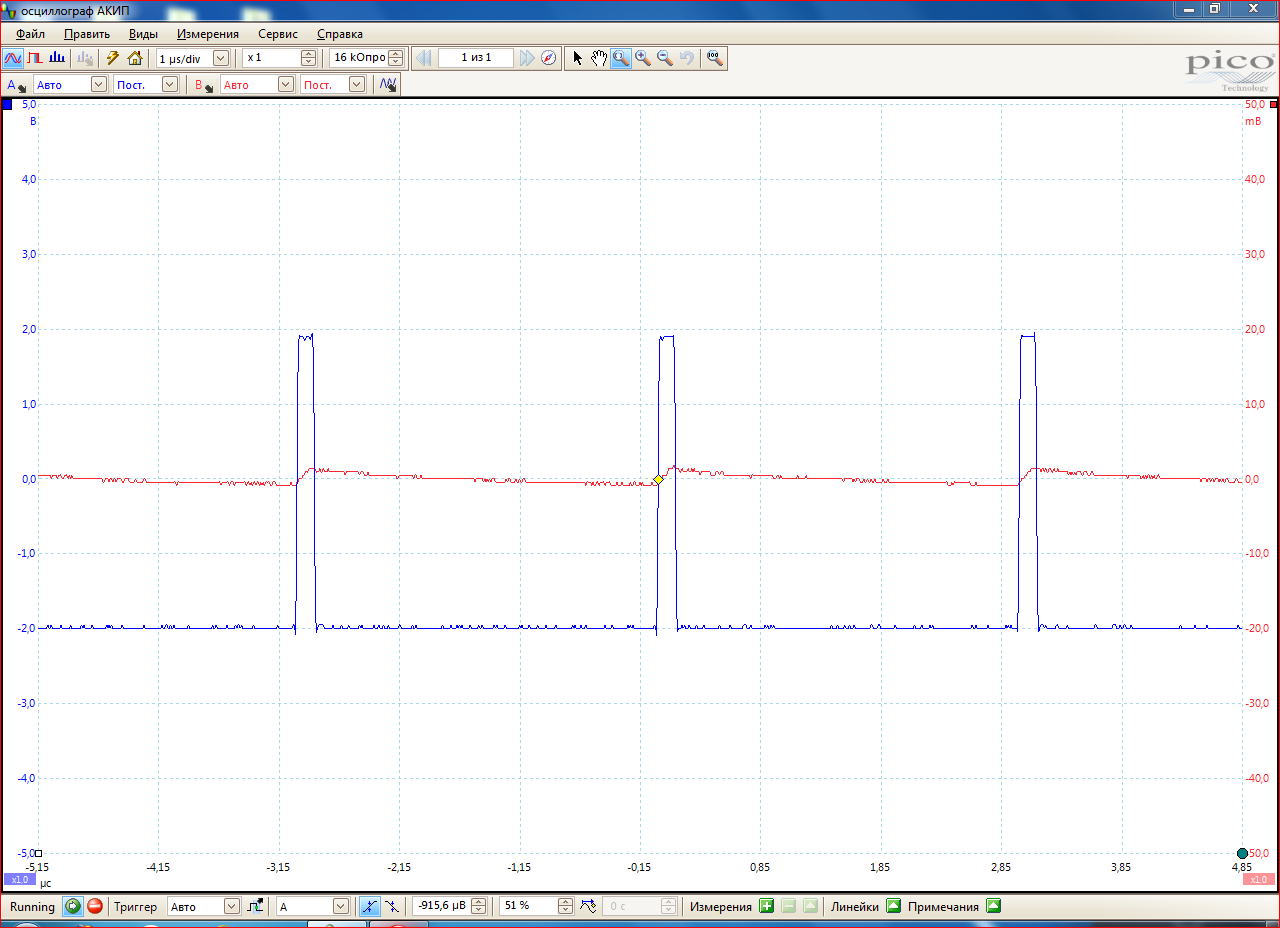
\includegraphics[width=0.95\linewidth]{img/data/F.27/3us_150ns.png}}
                        \caption{Прямоугольные импульсы\\($T = 3~мкс$; $\tau = 150~нс$)}
                        \label{plot:F.27.2}
                    \end{minipage}
                \end{figure}
                \begin{figure}[ht]
                    \begin{minipage}[ht]{0.49\linewidth}
                        \center{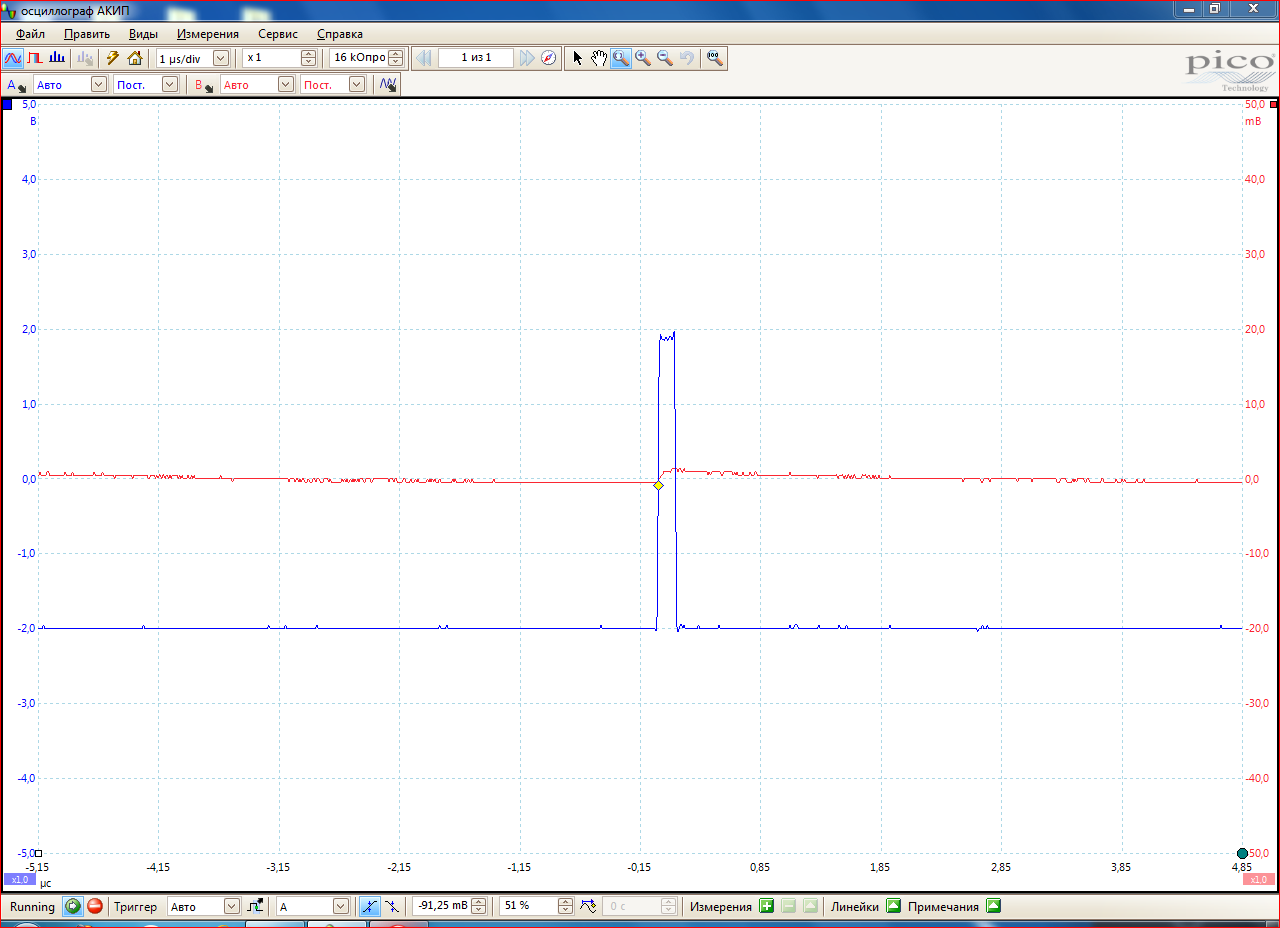
\includegraphics[width=0.95\linewidth]{img/data/F.27/6us_150ns.png}}
                        \caption{Прямоугольные импульсы\\($T = 6~мкс$; $\tau = 150~нс$)}
                        \label{plot:F.27.3}
                    \end{minipage}
                    \begin{minipage}[ht]{0.49\linewidth}
                        \center{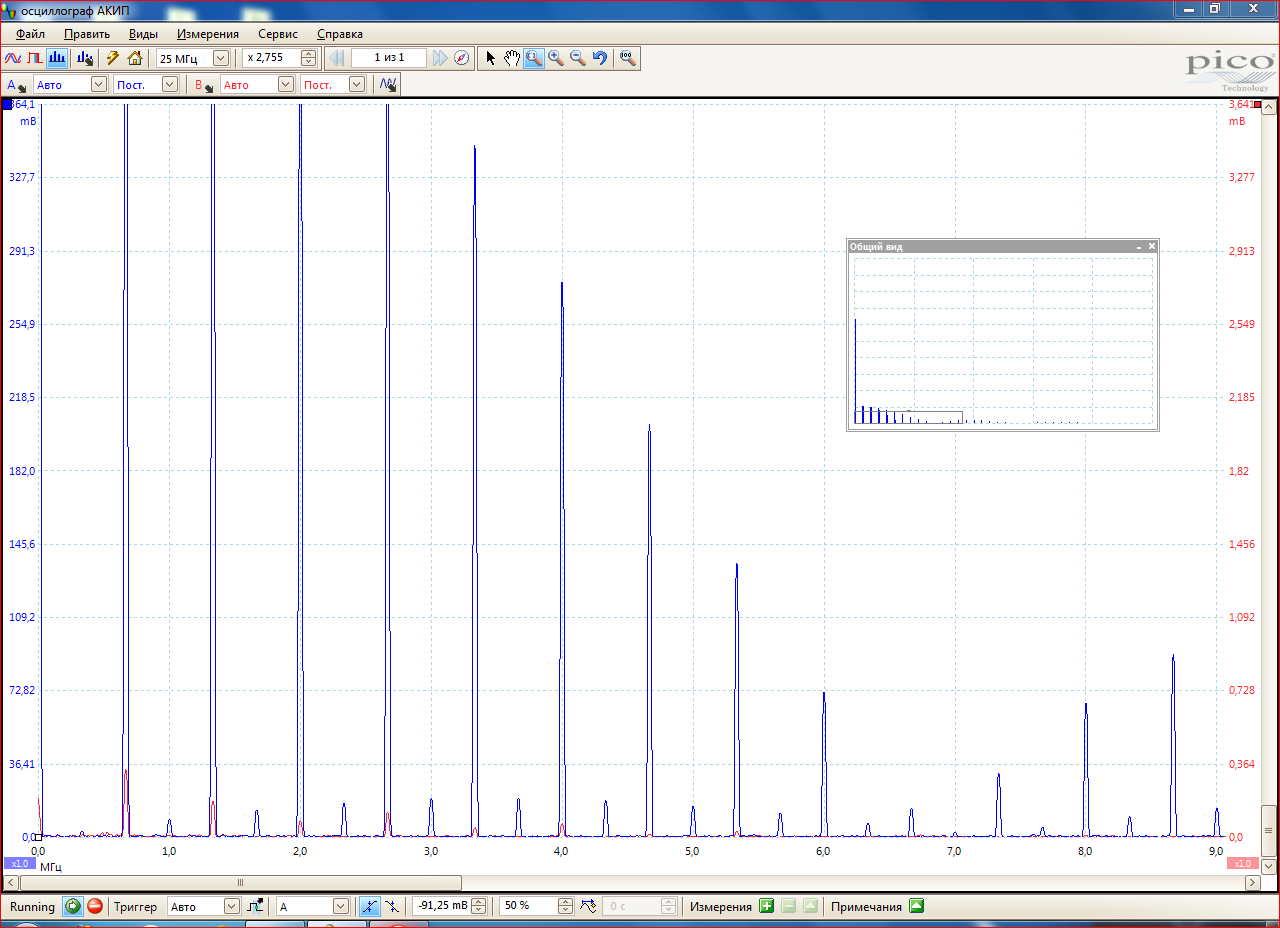
\includegraphics[width=0.95\linewidth]{img/data/F.27/1.5us_150ns_spectre.png}}
                        \caption{Спектр прямоугольных импульсов\\($T = 1.5~мкс$; $\tau = 150~нс$)}
                        \label{plot:F.27.4}
                    \end{minipage}
                \end{figure}
                \begin{figure}[ht]
                    \begin{minipage}[ht]{0.49\linewidth}
                        \center{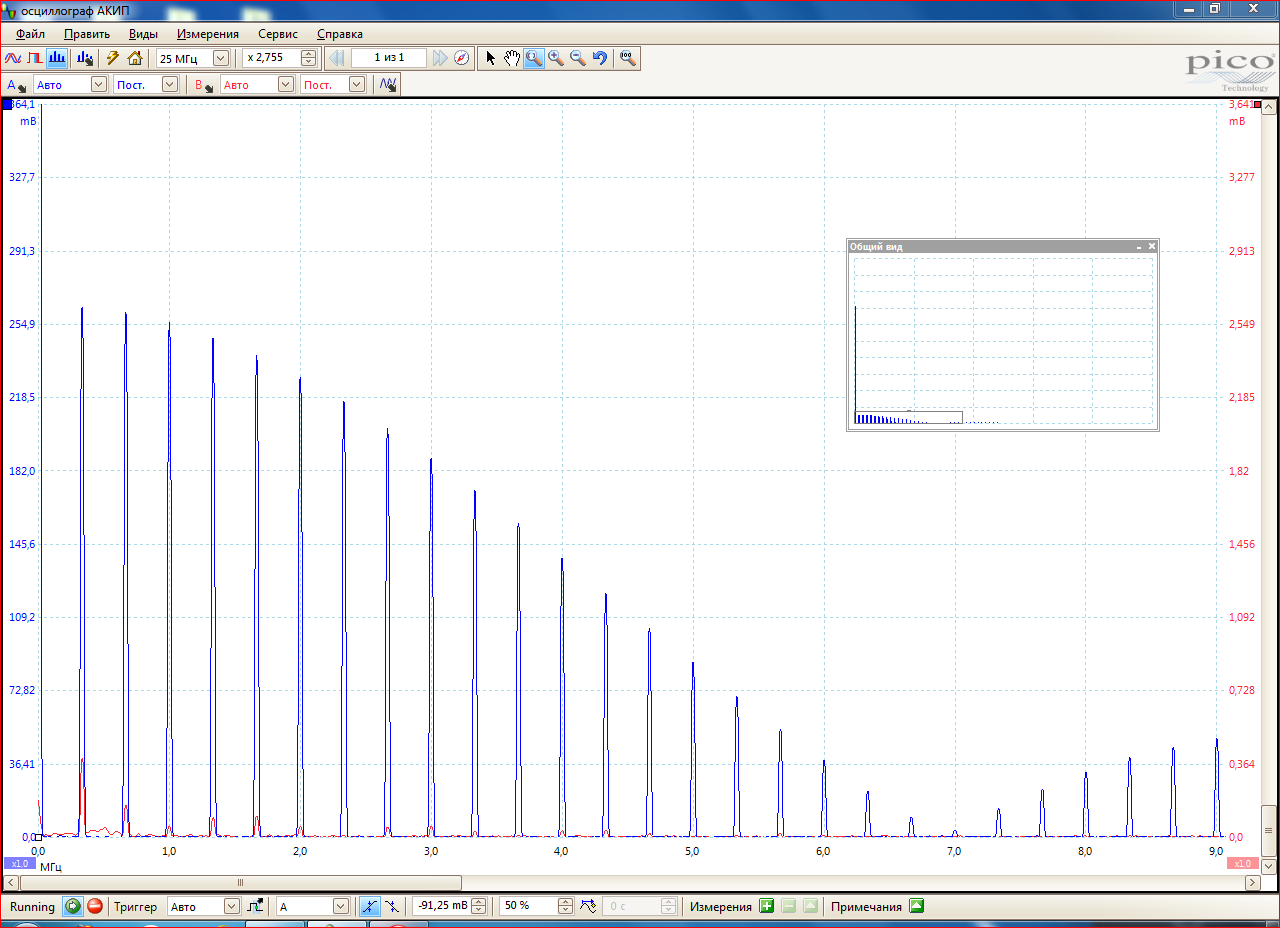
\includegraphics[width=0.95\linewidth]{img/data/F.27/3us_150ns_spectre.png}}
                        \caption{Спектр прямоугольных импульсов\\($T = 3~мкс$; $\tau = 150~нс$)}
                        \label{plot:F.27.5}
                    \end{minipage}
                    \begin{minipage}[ht]{0.49\linewidth}
                        \center{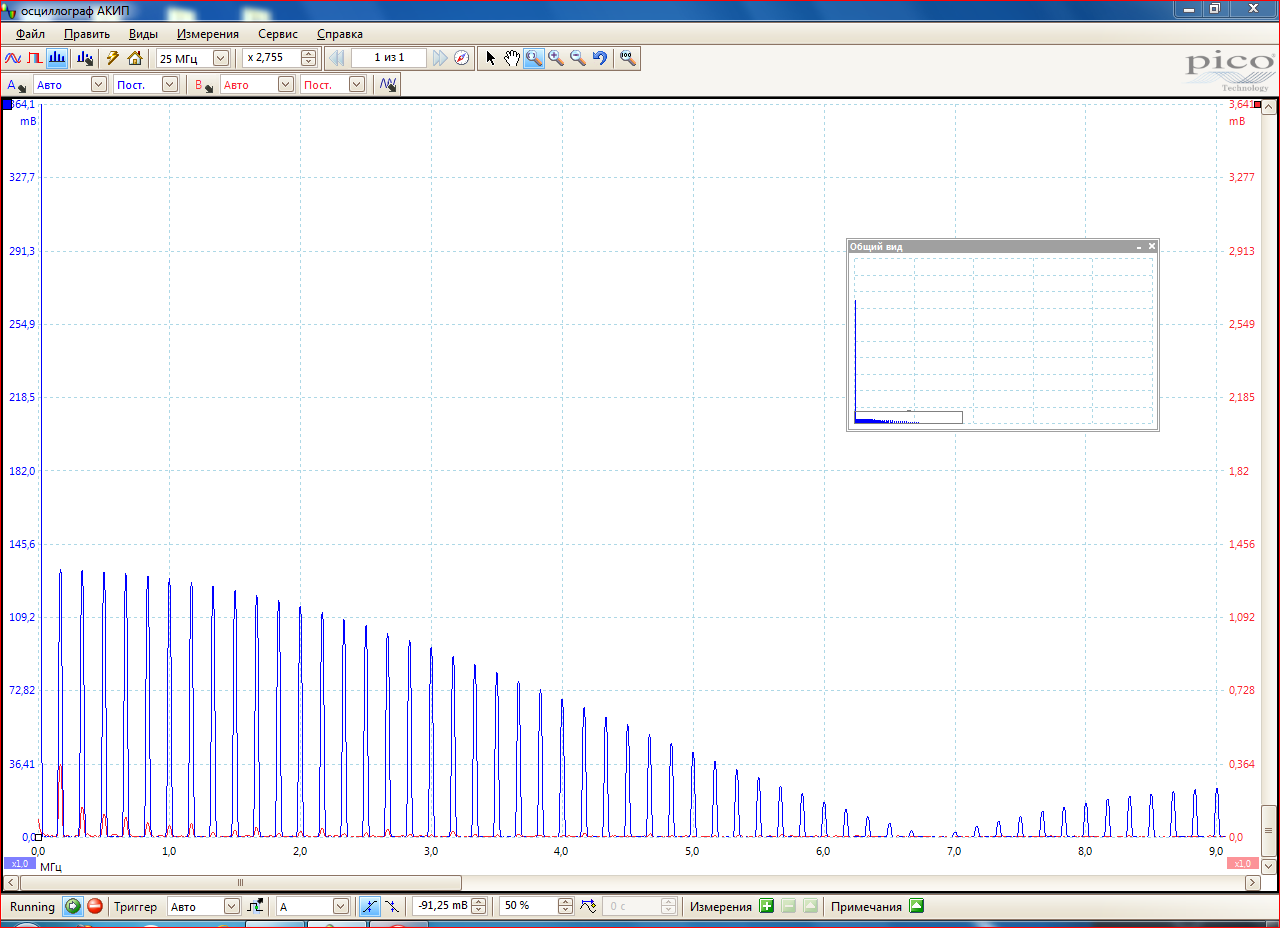
\includegraphics[width=0.95\linewidth]{img/data/F.27/6us_150ns_spectre.png}}
                        \caption{Спектр прямоугольных импульсов\\($T = 6~мкс$; $\tau = 150~нс$)}
                        \label{plot:F.27.6}
                    \end{minipage}
                \end{figure}

            \subsubsection{Сравнение амплитуд спектральных гармоник исходного и фильтрованного сигналов}

                Подадим последовательность прямоугольных импульсов с периодом повторения $T = 3~мкс$ и длительностью $\tau = 150~нс$

                Результаты измерения амплитуд фильтрованного и исходного сигнала в таблице \ref{tab:F.28}

                \begin{table}[!ht]
                    \centering
                    \begin{tabular}{|c|c|c|c|}
                        \hline

                        $n$ & $a_n^0, мВ$ & $a_n^ф, мВ$ & $K_n = \vert a_n^ф \vert / \vert a_n^0 \vert$\\ \hline
                        1 & $264 \pm 10$ & $33.5 \pm 1.0$ & $0.127 \pm 0.006$\\ \hline
                        2 & $260 \pm 10$ & $20.0 \pm 1.0$ & $0.077 \pm 0.005$\\ \hline
                        3 & $257 \pm 10$ & $9.6 \pm 1.0$ & $0.037 \pm 0.004$\\ \hline
                        4 & $247 \pm 10$ & $8.8 \pm 1.0$ & $0.036 \pm 0.004$\\ \hline
                        5 & $237 \pm 10$ & $8.8 \pm 1.0$ & $0.037 \pm 0.005$\\ \hline
                        6 & $227 \pm 10$ & $8.2 \pm 1.0$ & $0.036 \pm 0.005$\\ \hline
                        7 & $216 \pm 10$ & $6.4 \pm 1.0$ & $0.030 \pm 0.005$\\ \hline
                        8 & $202 \pm 10$ & $4.5 \pm 1.0$ & $0.022 \pm 0.005$\\ \hline
                        9 & $187 \pm 10$ & $2.0 \pm 1.0$ & $0.011 \pm 0.005$\\ \hline

                    \end{tabular}
                    \caption{Сравнение амплитуд спектральных гармоник исходного и фильтрованного сигналов}
                    \label{tab:F.28}
                \end{table}

                Теоретическая зависимость $K = \frac{1}{\tau_{RC}} \int_0^t f(t')dt'$

                Построим график $K(1/\nu)$ на рисунке \ref{plot:F.28}. По углу наклона определим $\tau_{RC}$

                \begin{figure}[ht]
                    \centering
                    \begin{minipage}[ht]{0.49\linewidth}
                        \center{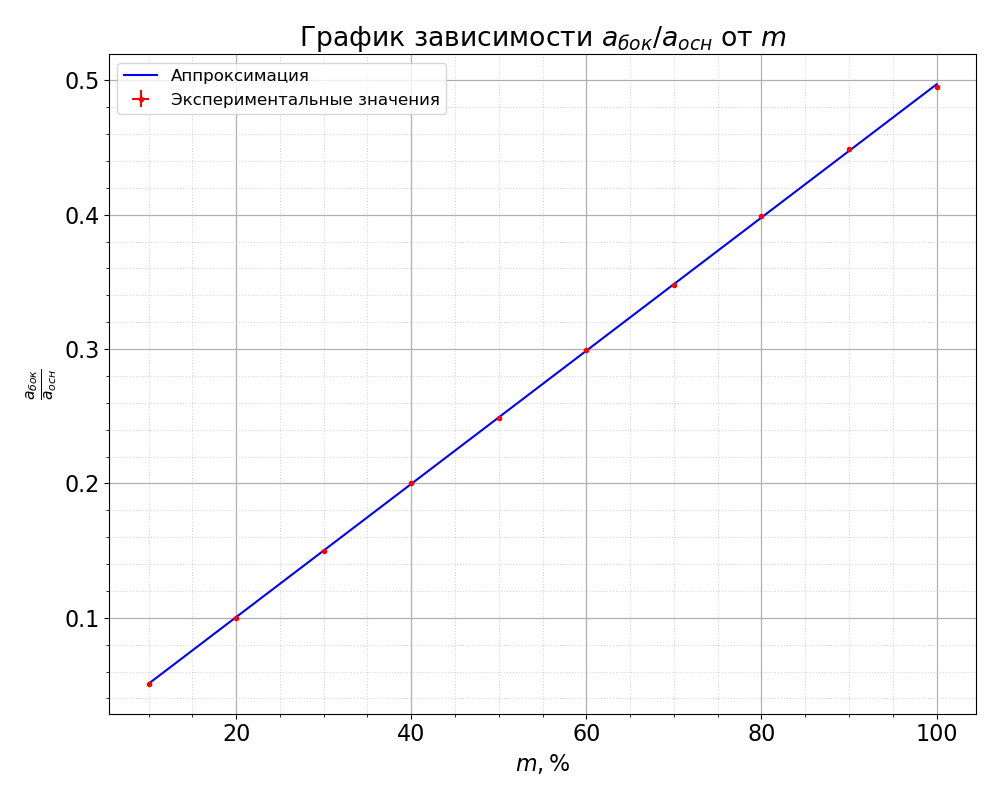
\includegraphics[width=0.95\linewidth]{img/plot_D.23.png}}
                        \caption{График зависимости $K(1/\nu)$}
                        \label{plot:F.28}
                    \end{minipage}
                \end{figure}

                $$
                    \tau_{RC} = \frac{1}{2 \pi k} = (3.6 \pm 0.6)~мкс
                $$

    \section{Вывод}

        В данной работе мы изучили понятие спектра и спектрального анализа, исследовали спектральный состав периодических электрических сигналов, а точнее прямоугольных импульсов, цугов гармонических колебаний, гармонических сигналов, модулированных по амплитуде и частоте, а также проанализировали фильтрацию сигналов при прохождении их через $RC$ контур. Проверили частный случай выполнения соотношения неопределённости.

\end{document}
